% Change to 'masters' to produces the masters thesis preliminary pages
\documentclass[oneside,masters,etd]{WSUclass}

\usepackage{import}

% preamble contains title page, signature page, acknowledgment and abstract texts
\usepackage{preamble}
\usepackage{bm}

% Pacakges used
\usepackage[utf8]{inputenc} % Remove warning on ascii conversion
\usepackage[T1]{fontenc} % Remove warning on ascii conversion
\usepackage[refsection=part,citestyle=apa,style=authoryear,natbib=true,backend=biber]{biblatex}
\usepackage{hyperref}
\usepackage{multirow}

% Make chapter numbers into string words 1 -> ONE
\usepackage{fmtcount}
\makeatletter
\renewcommand{\@makechapterhead}[1]{\vspace *{40\p@ }{\parindent \z@ 
\raggedright \normalfont \ifnum \c@secnumdepth >\m@ne \Huge \bfseries 
\@chapapp \space \Numberstring{chapter} \vskip 10\p@ \fi #1\par \nobreak \vskip 30\p@ }}
\makeatother

\addbibresource{bib.bib}

\newcommand\nt[1]{\textcolor{blue}{#1}}

\begin{document}

\hypersetup{breaklinks=true}

 % Start page counting in roman numerals
 \frontmatter

 % This command makes the formal preliminary pages.
 % You can comment it out during the drafting process if you want to save paper.
 %\makepreliminarypages

 \doublespace
 % Make the table of contents.
 \tableofcontents
 \thispagestyle{plain}

 % Make the list of tables
 \mylistoftables
 \thispagestyle{plain}
 
 % Make the list of figures
 \mylistoffigures
 \thispagestyle{plain}

  % This page is OPTIONAL. To remove, comment out and \dedicationpage in diss.tex
 %\dedicationpage
 \clearemptydoublepage

 % Start regular page counting at page 1
 \mainmatter

% OK. Everything is set up. Type your thesis here.
\addchapheadtotoc
\chapter{Context and related works}

In this chapter, we first introduce graphs and how they arise from real world networks. Then we present the graph classification problem, along with applications in which it arises. Finally, we proceed to detailing state-of-the-art methods and their limitations, before stating our contribution. 
 
\section{Graph structures and its presence in real world}

The need for graphs and their analysis can be traced back to 1679, when G.W.  Leibniz  wrote to C. Huygens about the limitations of traditional analysis methods of geometric figures and said that "we need yet another kind of analysis, geometric or linear, which deals directly with position, as algebra deals with magnitude", \citep{Graph_application}. This lead to graphs, mathematical objects that provide a pictorial and efficient form to represent data with many inter-connections. %With graph structures, these data become easier to be processed and analyzed, and that helps solving many problems that have been unsolved before \citep{Graph_application}.

Formally, a graph of size $v$ is a pair $\mathcal{G}=(\mathcal{V},\mathcal{E})$, where $\mathcal{V}=\{u_1,...,u_v\}$ is a set of $v$ graph nodes (or vertices), and $\mathcal{E}\in \mathcal{V}\times \mathcal{V}$ is the set of edges between these nodes, i.e. $(u_i, u_j)\in \mathcal{E}$ means that the graph has an edge between node $u_i$ and node $u_j$.

Graph structures are used to model a set of objects and their interactions/relations. % that link between different pairs of these objects.  
While the nature of these objects and their interactions vary with the application, the underlying modeling paradigm is the same for all applications: objects are represented by nodes, and a relation between two objects is represented by an edge between the corresponding two nodes. \nt{**For instance, in a social network like Facebook, nodes are .. and edges are... In a biological network such as the brain, nodes are brain regions and edges are.. In a transportation network such as the subway, nodes are .. and edges are.. (see Table.\ref{table:Graph_examples} for a list of different examples). } 

These graphs, if not too large, can be visually represented in order to provide an intuitive understanding of the existing interactions. Such an illustration is in Fig. \ref{fig:Graph_Example} in the application of chemical reactions.



\begin{figure}[H]
\centering
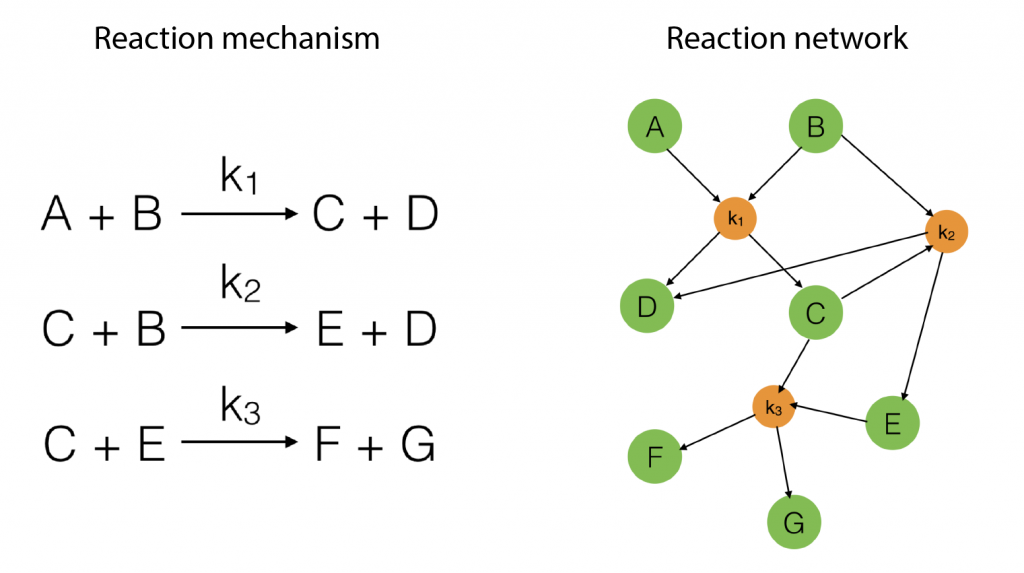
\includegraphics[scale=0.2]{figs/Graph_example.png}
\caption[Graph example to represent Chemical Reactions]{Graph structures in representing chemical reactions mechanisms}
%Source:
\label{fig:Graph_Example}
\end{figure}


\begin{table}
\small
\begin{center}
\begin{tabular}{|c|c|c|c|c|}
\hline
{Network}  &  {Nodes} & {Node features}  & {Edges}  & {Edge features}  \\
\hline
{Transportation System}  &  {cities} & {registered cars}  & {Routes}  & {Length, cost }  \\
\hline
{Banking Network}  &  {Account holders} & {account status}  & {Transactions}  & {Transaction value}  \\
\hline
{Social Network}  &  {users} & {name, country}  & {Interactions}  & {type (like, comment)}  \\
\hline
\end{tabular}
\end{center}
\caption{Some real world graphs}
\label{table:Graph_examples}
\end{table}

\section{Graph classification problem}
\label{sec:Graph_classification_problem}
Graph classification can be understood in several ways. Here, we place ourselves in the context of \emph{supervised learning}, where we suppose we have access to a set of pre-labeled graphs  $(\mathcal{X}=\{\mathcal{G}_1,\ldots,\mathcal{G}_n\}, \mathcal{Y}=\{y_1,\ldots,y_n\})$, where each graph $\mathcal{G}_i$ is \emph{a priori} known to belong to the class with label $y_i$. Stated simply, the graph classification problem we are interested in in this work may be stated as: given this prior information, design a classification algorithm that, given in input any graph (importantly, any graph belonging or not to $\mathcal{X}$), outputs the label of the class to which it belongs. 

More formally, consider the set $\mathcal{D}$ of all graphs $\mathcal{G}$ that can occur in some real-world application, a fixed set of classes $\beta=\{\beta _1,\ldots,\beta _l\}$ of finite size $l$, and a mapping function $f:\mathcal{D}\mapsto\beta$ which maps each graph $\mathcal{G}$ in $\mathcal{D}$ to the class $\beta_\mathcal{G}$ it belongs to. Graph classification is the problem of estimating the mapping function $f$ in the case where it is only known on a subset $\mathcal{X}\subset \mathcal{D}$. Formally, we have a dataset $(\mathcal{X}=\{\mathcal{G}_1,\ldots,\mathcal{G}_n\}, \mathcal{Y}=\{y_1,\ldots,y_n\})$ of size $n$ such that $\mathcal{X}\in \mathcal{D}^n$ and $\mathcal{Y}\in\beta^n$, where for each graph $\mathcal{G}_i\in \mathcal{X}$ we have that $y_i=f(\mathcal{G}_i)$ is the class of $\mathcal{G}_i$. The classification task is to have a \textbf{predictive model} which can predict well, based on some-predefined metric,  the class for any new graph $\mathcal{G}$ in $\mathcal{D}$. This prediction functionality of the model is gained using the dataset $(\mathcal{X}, \mathcal{Y})$ to optimize the parameters of the model that is believed to govern the behavior of the mapping function $f$ on $\mathcal{D}$. This optimization completed in this paradigm is called the learning algorithm.

Note that graph classification as considered here, has nothing to do with the more common problem of \emph{node classification} in a graph, in which there exists only one graph and the goal is to separate the node set in a partition of communities. In our work, graphs are classified, not nodes. This being said, the extra information that the nodes and/or edges may have in some applications (gender, age for instance for nodes of a social network; maximum bandwidth, number of channels for instance for edges of a communication network; etc.) could in principle be used along with the graph structure to classify different graphs into different classes. However, as the existence of such extra-information is very application-dependent, we prefer to focus here on the case where nodes and edges do not carry such information: the only information one has access to for classification is the graph structure.

This problem has been addressed in many different fields of research, such as:
\begin{itemize}
    \item \textbf{\emph{Marketing analytics:}} advertisers and marketers  are interested in detecting the influential people communities in Social Networks in the sense that addressing their products' advertisements to such groups would be a more rewarding investment. This can be approached with graph classification applied on these networks \citep{marketing_analytics}.
    \item \textbf{\emph{Banking security:}} graph classification is used to catch unusual patterns of fraudulent transactions \citep{banking_security}.
    \item \textbf{\emph{Biology and genomics:}} graphs are based on proteins such that nodes correspond
to amino acids which compound the protein and a pair of amino acids are linked by an edge if they are less than 6 Angstroms apart. The task is to detect whether a protein is an enzyme or not \citep{protein_application}, to mention a few.
\end{itemize}

\section{State-of-the-art methods for graph classification}
\label{section:state}
We  present here existing algorithms for the graph classification problem and discuss their limitations. In general, these algorithms can be classified in four main categories: set based, frequent sub-graph based, kernel based, and graph neural networks based algorithms.\\

\noindent\textbf{Set based algorithms.} This type of algorithms is only applicable to cases where nodes/edges are supplied with features or attributes, as they completely disregard the graph's structure. Based on the provided feature vectors, a distance function of interest between the graphs is computed. % in order to provide a similarity between pairs of edges/nodes in the corresponding sets. 
The drawback of this method is that it does not take the structure (topology) of the graph itself into consideration. For example, if we just compare how much the edges' features of one graph are similar to the edges' features of another, we can have two graphs with the same set of edge features, which will lead to maximum similarity, even though their graph structures can be arbitrarily different. %but we in reality ignore other important information that can make these graphs completely different. % such as how many connected communities of nodes these edges form in each graph, how many circles of nodes these edges promote in each graph, etc. 
On the other hand, a strength of these algorithms is their low computations cost that is usually linear or quadratic in the number of nodes and edges \citep{graphlet_kernel}.\\
 
\noindent\textbf{Frequent sub-graph based algorithms.} These algorithms contain two steps. First, the graph dataset $\mathcal{X}$ is analyzed to enumerate the frequent sub-graphs occuring in the different graphs. Then, another analysis is done to choose the most discriminative sub-graphs out of the ones found during the first step. The disadvantage of using this method is the computational cost that grows exponentially with the graph size \citep{graphlet_kernel}. \\

\noindent\textbf{Graph kernels based algorithms.} It is a middle ground between both previous methodologies, where the graph structure is well considered, and in most cases, these algorithms are designed in a way that the computational time is a polynomial function of the graph size \citep{graphlet_kernel}. However, some effective and competitive kernels still require exponential time, and this is in short the problem we approach in this work using random features to approximate these kernels or to compete with them in notably lower computational time. \\

\noindent\textbf{Graph neural networks (GNNs) based algorithms.} GNNs compute a representation vector (embedding vector) for every node in a graph, where this vector is recursively computed by aggregating the representation vectors of neighboring nodes. The goal of this aggregation technique is that nodes that are neighbors (or close) to each other in the graph are more likely to have similar representations (with respect to some similarity function) and vice versa. On the graph level, a representation vector is computed by aggregating its nodes' representation vectors. This aggregated vector now representing the graph itself is used as a usual feature vector which can be fed to a typical deep neural network to learn the classification task. Traditional GNNs such as graph convolutional networks (GCNs) and GraphSAGE fail to provide high performance classifying graphs whose node/edges don't include any original feature vectors, and that even applies on graphs with simple topology \citep{GCN_powerful}. \nt{I could not re-write this last sentence: I don't understand it} 
However, another GNN structure was developed to overcome this weakness point \nt{complete failure is more than a ``weakness''}, and it is referred to by Graph Isomorphism Network (GIN). Regarding the computational time, it is mainly a matter of the layers number in the network, since this parameter in reality represents how far from a node we want to go in order to compute its representation vector. 

\section{Our contribution}
One of the methods of the kernel-based algorithms (the third out of the four categories listed), called graphlet kernel, has proven to be competitive for graph classification. Theoretically and empirically, it was shown that a desired performance or a required amount of information to be preserved from the original graph can be reached with sufficiently large $k$. \nt{**hold your horses! we need at least a few sentences actually \emph{explaining} what is the graphlet kernel you are talking about. For instance, we have yet no clue what $k$ is.**}
However,  the computational cost  becomes prohibitive as $k$ (the graphlet size) and/or $v$ (the size of the graph)  become too large. Thus it cannot be applied on large-scale graph datasets. 

The advent of Optical Processing Units (OPUs) opened a new horizon solving this problem, since it can apply enormous number of \emph{Random Projections} in light speed. \nt{**hold your horses! The reader has no clue \emph{why} making random projections in light speed is actually useful for your problem. You need at least one sentence explaining what you mean by random projections}

In this work, we did the sufficient mathematical analysis to prove that OPUs' light-speed random feature projections compete the $k$-graphlet kernel with respect to \emph{Maximum Mean Discrepancy (MMD)} Euclidean metric. Moreover, we empirically tested this hypothesis and made sure that the the theoretical MMD error is aligned with the empirical one with respect to the parameters introduced in the problem (sampling technique, number of sampled sub-graphs, number of random features, etc). \nt{Instead of this last paragraph, I invite you to write ``Our contributions are the following:'' followed by an ``enumerate'' environment to make a clear and thorough list of your achievements. After that enumeration, I invite you to write ``On top of these contributions, we have also:'' followed by an ``enumerate'' environment to make a list of things you did that we cannot call ``contributions'' yet as they either did not work or are work in progress.}






\newcommand{\todoNK}[1]{\textbf{\textcolor{red}{NK: #1}}}
\chapter{Background}
\label{chapter:background}
\newtheorem{theorem}{Theorem}
In this chapter we present the necessary background that the reader should have in order to proceed through the next two chapters, which are the core of this work. After a brief overview of kernel methods in machine learning, we will present random features and graph kernels. In the next chapter, these different notions will be combined in the proposed algorithm.

\section{Kernel methods and random features}

We first start by an overview of kernel methods.

\subsection{Kernel methods and kernel trick}
Kernel methods is a family of classic algorithms in machine learning that learn models as a combination of similarity functions between data points $(x,x')$, defined by positive semi-definite (psd) \emph{kernels} $\kappa(x,x')$. Denote by $\mathcal{D}$ the set of all possible data points. A symmetric function $\kappa:\mathcal{D}\times\mathcal{D}\mapsto\mathbb{R}$ is said to be a positive semi-definite kernel if:
\begin{equation}
\forall n\in \mathbb{N},~\forall \alpha_1,\ldots,\alpha_n\in \mathbb{R},~\forall x_1,\ldots,x_n\in \mathcal{D},\quad \sum_{i,j}^n\alpha_i\alpha_j\kappa(x_i,x_j)\geq 0 \, .
\end{equation}
Let us now illustrate how kernels can be incorporated to learning models and how that is useful to learn more complex functions. To do that let us consider a classical supervised learning setting for classification: take $\mathcal{D}=\mathbb{R}^d; d\in\mathbb{N}$, and let $\mathcal{X}=(\mathbf{x}_1,\ldots,\mathbf{x}_n)$ be a set of $n$ datapoints in $\mathbb{R}^d$, along with the vector of their associated known labels $\mathbf{y}=(y_1,\ldots,y_n)^T\in\mathbb{R}^n$ where, for each $i$, $y_i$ is the label of the class to which $\mathbf{x}_i$ belongs. For simplicity, we set ourselves in the context of two classes, and we set $y_i=-1$ if $\mathbf{x}_i$ belongs to class $1$, and $y_i=1$ if $\mathbf{x}_i$ belongs to class $2$. 

The classification task is: given this \emph{a priori} known labeled data $(\mathcal{X},\mathbf{y})$, design a classifier that is able to classify any new data point in $\mathbb{R}^d$. 

Many learning models designed to solve this problem, like Support Vector Machine (SVM) \citep{svm_tut}, and Perceptron binary classifier \citep{perceptron_tut}, rely on the inner product as a measure of similarity between data points: during the training, they only use inner products $\mathbf{x}_i^T \mathbf{x}_j$, and then produce classifiers with the following form \citep{inner_product}:
\begin{equation}
\label{eq:inner_product}
\hat{y}(\mathbf{x})=\text{sign}\left\{\sum_{i=1}^n\alpha_iy_i\mathbf{x}_i^T\mathbf{x}\right\} \text{ with } \alpha_i\in \mathbb{R}
\end{equation}
where the values $\{\alpha_i\}_{i=1,\ldots,n}$ in Eq. \ref{eq:inner_product} are optimized based on the dataset $(\mathcal{X},\mathbf{y})$ by the learning algorithm. The intuition behind Eq. \ref{eq:inner_product} is that the output class for every new data point $\mathbf{x}$ is expected to be the same class of nearby points in the input set $\mathcal{D}$. This is achieved by introducing the inner product $\mathbf{x}_i^T\mathbf{x}$ to control how much the class $y_i$ contributes in the output $\hat{y}(\mathbf{x})$. The parameter $\alpha_i$ controls how strongly the data point $x_i$ can affect other neighboring points. They mainly depend on how both classes are distributed in the input set $\mathcal{D}$, and  how much the dataset $(\mathcal{X},\mathbf{y})$ is noisy. 



A \emph{kernel method} consists in replacing every inner products $\mathbf{x}_i^T \mathbf{x}_j$ by a psd kernel $\kappa(\mathbf{x}_i, \mathbf{x}_j)$ during training, and similarly $\mathbf{x}_i^T\mathbf{x}$ by $\kappa(\mathbf{x}_i, \mathbf{x})$ during prediction.
Let us now explain the intuition behind this, starting by rewriting Eq. \ref{eq:inner_product} as 
\[
\hat{y}(\mathbf{x})=\text{sign}\{\textbf{x}^T(\mathbf{X}^T~diag([\alpha]_{i=1}^n)~\mathbf{y})\},
\]
where $\mathbf{X}\in\mathbb{R}^{n\times d}$ is the matrix whose $i$-th row corresponds to data-point $\mathbf{x}_i$, and where $diag([\alpha]_{i=1}^n)$ is the diagonal matrix with values $[\alpha]_{i=1}^n$. 

To get the decision boundary of such classifiers (the boundary in $\mathbb{R}^d$ that separates $\mathbb{R}^d$ into a part associated to class 1 and another associated to class $2$), one solves $\mathbf{x}^T\mathbf{q}=\mathbf{0}$, where $\textbf{q}=(\mathbf{X}^T~diag([\alpha]_{i=1}^n)~\mathbf{Y})\in\mathbb{R}^d$. It is the equation of a hyper-plane in the input space $\mathbb{R}^d$, also referred to as a \emph{linear} decision boundary. 
The question here is: what if the two classes are not separable by a hyper-plane (as illustrated on the left of Fig. \ref{fig:SVM_boundaries})? 

\begin{figure}[t]
	\centering
	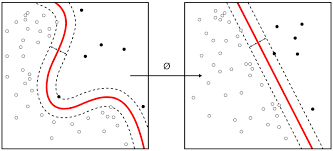
\includegraphics[scale=0.8]{figs/svm.png}
	\caption[The case where classes aren't separable using linear boundary]{The left figure shows a case where the input data in their original space are not separable by a linear boundary. The right figure shows another input dataset where different classes are separable using linear boundary. }
	\label{fig:SVM_boundaries}
\end{figure}

One common solution to this problem is to map the data points from $\mathbb{R}^d$ to another space $\mathbb{R}^m$  through a proper mapping function $\varphi$ such that the two classes become separable with a linear decision boundary in $\mathbb{R}^m$. Then we can apply the same learning models specified in Eq. \ref{eq:inner_product} but on the transformed data. Let us consider for example the dataset shown in Fig. \ref{fig:polynomial_kernel},  we can use the following mapping function $\varphi:(x_1,x_2)\mapsto (\sqrt{2}x_1x_2,x_1^2,x_2^2)$ to move from $\mathbb{R}^2$ on the left, where data are not linearly separable, to $\mathbb{R}^3$ on the right, where they are.

\begin{figure}[H]
	\centering
	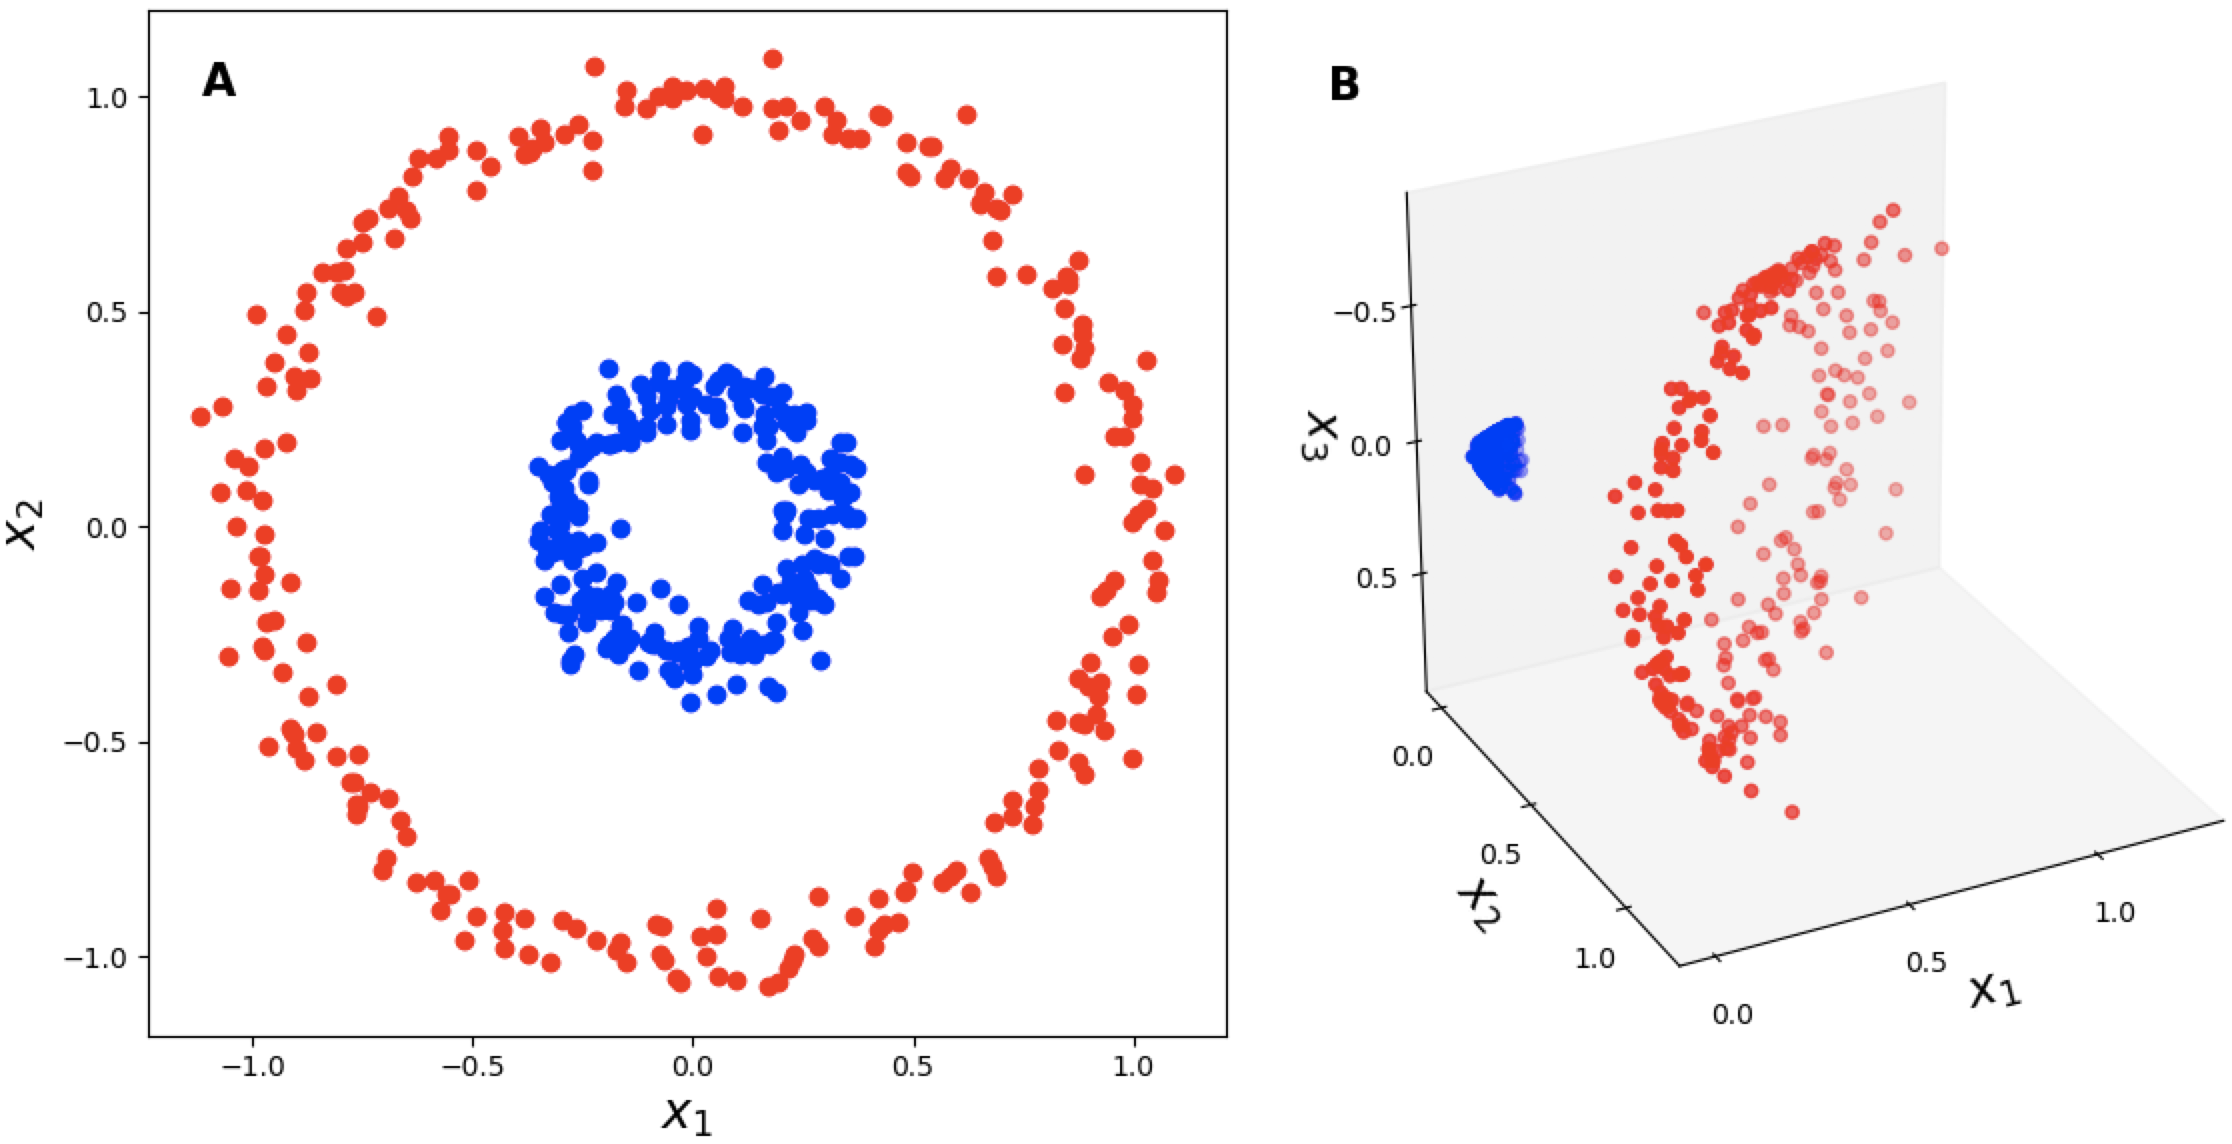
\includegraphics[scale=0.25]{figs/poly_kenrnel.png}
	\caption[Lifting data to a higher-dimension space to get linearly separable classes]{ Using the mapping function $\varphi:(x_1,x_2)\mapsto (\sqrt{2}x_1x_2,x_1^2,x_2^2)$ to map the data on the left from $\mathbb{R}^2$ to $\mathbb{R}^3$ where they are linearly separable}
	%Source:
	\label{fig:polynomial_kernel}
\end{figure}

Learning such a function $\varphi$ is what is typically done by neural networks using complex optimization methods.  Kernel methods are much simpler (and elegant) methods to perform this mapping. They are justified by the following key theorem.

\begin{theorem}[Mercer theorem]
	To every positive semi-definite kernel $\kappa:\mathbb{R}^d\times \mathbb{R}^d\mapsto \mathbb{R}$, there exists a Hilbert space $\mathbb{H}$ and a feature map $\phi:\mathbb{R}^d\mapsto\mathbb{H}$ such that for all $\mathbf{x},\mathbf{x}'\in\mathbb{R}^d$ one has:: 
	\begin{equation}
	\label{eq:kernel_main_equation}
	\kappa(\mathbf{x},\mathbf{x}')=<\phi(\mathbf{x}),\phi(\mathbf{x}')>_\mathbb{H}
	\end{equation}
	where $<\phi(\mathbf{x}),\phi(\mathbf{x}')>_\mathbb{H}$ is the inner product defined in $\mathbb{H}$.
\end{theorem}

This theorem states that replacing the inner product $\mathbf{x}_i^T\mathbf{x}$ in Eq. \ref{eq:inner_product} by a positive semi-definite kernel $\kappa(\mathbf{x}_i,\mathbf{x})$ is equivalent to implicitly map the data from the original input space $\mathcal{D}$ to another feature space $\mathbb{H}$ and then apply the classical inner product. Therefore, one \emph{does not need to know explicitely the mapping} $\phi$ nor the new feature space $\mathbb{H}$, instead, it is sufficient to evaluate the kernel $\kappa$ for pairs of data points in the original input space $\mathcal{D}$. This main feature of kernel methods is known as the \emph{kernel trick}. It has two main advantages:
\begin{itemize}
	\item Kernels allow us to transform data to a new Hilbert space of very high or even infinite dimensionality, which can make the learning model able to represent more complex functions.
	\item Kernels are often computationally cheaper, since they save the time required to compute the explicit co-ordinates of the data in the new feature space by directly calculating the inner product between the transformed data.
\end{itemize}
To better illustrate these benefits, we take the Gaussian kernel as an example, which is one of the most classical kernels in $\mathbb{R}^d$, defined as:
\begin{equation}
\label{eq:Guassian_kernel}
\kappa_{G}(\mathbf{x},\mathbf{x}')=\exp^{-\frac{\left \| \mathbf{x}-\mathbf{x}'\right\|^2}{2\sigma^2}}
\end{equation}
where $\sigma>0$ is the bandwidth parameter of the kernel. The lifting function $\phi_G$ of this kernel is located in a Hilbert space of infinite dimension \citep{kriege_graph_kernels}, but the kernel can be easily evaluated for any pair $(\mathbf{x},\mathbf{x}')\in\mathbb{R}^d\times \mathbb{R}^d$.

Despite their advantages, kernel methods still have some drawbacks, notably in the computation of the Gram matrix. The Gram matrix associated to a given kernel $\kappa$ and a given set $\mathcal{X}$ of $n$ datapoints in $\mathbb{R}^d$, is a matrix of size $n\times n$ whose $(i,j)_{th}$ entry equals the kernel evaluated between points $\mathbf{x}_i$ and $\mathbf{x}_j$: $\kappa(\mathbf{x}_i, \mathbf{x}_j)$. This Gram matrix is typically needed to learn the parameters $\{\alpha_i\}$ of the classifier. Computing this matrix takes however $\mathcal{O}(dn^2)$ operations. As $n$ and/or $d$ increase, this computation cost may become prohibitive. 

%\begin{itemize}
%   \item The Gram matrix associated to a given kernel $\kappa$ and a given set $\mathcal{X}$ of $n$ datapoints in $\mathbb{R}^d$, is a matrix of size $n\times n$ whose $(i,j)_{th}$ entry equals the kernel evaluated between points $\mathbf{x}_i$ and $\mathbf{x}_j$: $\kappa(\mathbf{x_i}, \mathbf{x_j})$. This Gram matrix is typically needed to learn the parameters $\{\alpha_i\}$ of the classifier. Computing this matrix takes however $\mathcal{O}(dn^2)$ operations and requires $\mathcal{O}(n^2)$ memory space. As $n$ and/or $d$ increase, these computation time and memory costs may become prohibitive. 
%   Since for most kernels we need to evaluate the kernel on each pairs of data points, for a dataset $(\mathbf{X},\mathbf{X})$ \nt{?} of size $n$, we need $O(n^2)$ memory entries to compute what is called a Gram matrix, .
%   \item Even if most kernels are designed so that they can be evaluated in polynomial time in the dimensionality of the input space $\mathcal{D}$ (for instance computing $\mathcal{K}_{G}(\mathbf{x},\mathbf{x}')$ for two vectors in $\mathbb{R}^d$ costs $d$ operations),  some kernels (especially on graphs) are computationally expensive \citep{graphlet_kernel}. \todoNK{I would not mention that here, since handling exponential computation of *each individual evaluation* of the kernel with RF is precisely what we do which has not been done before. Only the Gram matrix problem is mentioned in the original RF paper.}
%\end{itemize}

To overcome these difficulties, random feature projections is a technique developed to approximate kernels, often requiring less computational time and less memory storage.

\subsection{Random features}
\label{sec:RF}
Random features (RF) \citep{rahimi2008random} is an approach developed to approximate kernel methods with reduced computational time. The idea is that, instead of considering the true lifting function $\phi$ in Eq. \ref{eq:kernel_main_equation}, we explicitly map the data points using an appropriate randomized feature map $\varphi:\mathcal{D} \xrightarrow{}\mathbb{C}^m$, such that the kernel evaluated for two data points $\mathbf{x}, \mathbf{x}'$ is approximated by the inner product of their random features with high probability:
\begin{equation}
\label{eq:approx_RF}
\kappa(\mathbf{x},\mathbf{x}')=<\phi(\mathbf{x}),\phi(\mathbf{x}')>_\mathbb{H} \approx \varphi(\mathbf{x})^*\varphi(\mathbf{x}')
\end{equation}
where $^*$ stands for the conjugate transpose. 
Considering this approximation, we can transform the input vectors of $\mathcal{X}$ with $\varphi$ and then apply a linear learning method as in Eq. \ref{eq:inner_product} to have a similar learning power as the original non-linear kernel machine, while often avoiding the cost of explicitly constructing the Gram matrix. Note that with RF we do not use the kernel trick anymore, but construct an explicit (even if random) mapping $\varphi$ to approximate the kernel $\kappa$.

Most RF constructions are known as Random \emph{Fourier} Features (RFF), and are based on the following theorem.
\begin{theorem}[Bochner's theorem]
	A continuous and shift-invariant kernel $\kappa(\mathbf{x},\mathbf{x}')=\kappa(\mathbf{x}-\mathbf{x}')$ on $\mathbb{R}^d$ is positive definite if and only if $\kappa$ is the Fourier transform of a non-negative measure.
\end{theorem}
As a direct consequence, we can easily scale any shift-invariant kernel to obtain $\kappa(0) = \int p = 1$, so that its Fourier transform $p(\mathbf{w})$ is a correct probability distribution. We obtain that any shift-invariant psd kernel is of the form:
\begin{equation}
\label{Fourier integral}
\kappa(\mathbf{x}-\mathbf{x}')=\int_{\mathbb{R}^d}p(\mathbf{w})e^{j\mathbf{w}^T(\mathbf{x}-\mathbf{x}')}d\mathbf{w}= E_{\mathbf{w}\sim p}[\xi_\mathbf{w}(\mathbf{x})^*\xi_\mathbf{w}(\mathbf{x}')]
\end{equation}
where $\xi_\mathbf{w}(\mathbf{x})=e^{-j\mathbf{w}^T\mathbf{x}}$ and where $E_{\mathbf{w}\sim p}$ stands for the expectation over $\mathbf{w}$ drawn from the probability distribution $p(\mathbf{w})$. Note that, since $\kappa$ is a real-valued function, from Eq.~\ref{Fourier integral} one can also prove that:
\begin{equation}
\label{real Fourier integral}
\kappa(\mathbf{x}-\mathbf{x}')=\int_{\mathbb{R}^d}p(\mathbf{w})cos({\mathbf{w}^T(\mathbf{x}-\mathbf{x}')})d\mathbf{w}=E_{\mathbf{w}\sim p}[\tilde \xi_\mathbf{w}(\mathbf{x})\tilde \xi_\mathbf{w}(\mathbf{x}')]
\end{equation}
where $\tilde \xi_\mathbf{w}(\mathbf{x})=\sqrt{2}cos(\mathbf{w}^T\mathbf{x}+b)$ such that $\mathbf{w}$ is drawn from $p$ and $b$ is drawn uniformly from $[0,2\pi]$. So here we can use a real-valued mapping if desired.

As a result, for $\mathbf{w}$ a random variable drawn from $p(\mathbf{w})$, $\  \xi_\mathbf{w}(\mathbf{x})^*  \xi_\mathbf{w}(\mathbf{x}')$ is an unbiased estimate of $\kappa(\mathbf{x},\mathbf{x}')$. The RF methodology consists in averaging $m$ instances of the estimator with different random frequencies $\mathbf{w}_j$ drawn identically and independently (iid) from $p$, that is, define
\begin{align}
	\label{eq:def_RF}
	\varphi(\mathbf{x}) = \frac{1}{\sqrt{m}} ( \xi_{\mathbf{w}_j}(\mathbf{x}) )_{j=1}^m \in \mathbb{C}^m
\end{align}
such that $\varphi(\mathbf{x})^*\varphi(\mathbf{x}')=\frac{1}{m} \sum_{j=1}^m \xi_{\mathbf{w}_j}(\mathbf{x})^*\xi_{\mathbf{w}_j}(\mathbf{x}')$, which converges to $\kappa(\mathbf{x},\mathbf{x}')$ by the law of large numbers. Moreover, Hoeffding's inequality guarantees exponentially fast convergence in $m$ between $\varphi(\mathbf{x})^*\varphi(\mathbf{x}')$ and the kernel's true value:
\begin{equation}
\forall \epsilon >0\qquad Pr(|\varphi(\mathbf{x})^*\varphi(\mathbf{x}')-\kappa(\mathbf{x},\mathbf{x}')|\geq\epsilon)\leq2e^\frac{-m\epsilon^2}{4},
\end{equation}
that is, for any error $\epsilon>0$, the probability that the estimation is off by more than $\epsilon$ is controlled by an exponentially decaying term.

One could use the union bound on all couples $(\mathbf{x},\mathbf{x}')\in\mathcal{X}^2$ to study the  concentration of \emph{all} entries of the Gram matrix, not only a given couple as in the previous Hoeffding inequality:
\begin{theorem}[]\label{thm:RF_vs_logn}
	Let $\epsilon\in(0,1)$ and $\delta\in(0,1)$. Consider a dataset $\mathcal{X}=(\mathbf{x}_1,\ldots,\mathbf{x}_n)$ of $n$ elements, and a psd shift-invariant kernel $\kappa$. The random embedding  $\varphi(\mathbf{x})\in\mathbb{C}^m$ defined in Eq.~\eqref{eq:def_RF} enables a controlled approximation of \emph{all} the elements of the Gram matrix with probability larger than $1-\delta$, \emph{i.e.}
	$$\text{Pr}\left(\forall (\mathbf{x}, \mathbf{x}')\in\mathcal{X}^2\quad|\varphi(\mathbf{x})^*\varphi(\mathbf{x}')-\kappa(\mathbf{x},\mathbf{x}')|\leq\epsilon\right)\geq 1-\delta$$ 
	provided that 
	$$m\geq\mathcal{O}\left(\frac{1}{\epsilon^2}\log{\frac{n}{\delta}}\right).$$
\end{theorem}

As an illustration, consider the Gaussian kernel in Eq. \ref{eq:Guassian_kernel}. This kernel is shift-invariant and known to be positive semi-definite. It is already correctly normalized since $\kappa(0) = 1$, and its Fourier transform is also a Gaussian but with inverted variance:
\begin{equation}
\label{eq:G_fourier}
    p(\mathbf{w})=FT\big(\kappa_G\big)(\mathbf{w})=\left(\frac{\sigma^2}{2\pi}\right)^\frac{d}{2}e^{-\frac{\sigma^2\|\mathbf{w}\|^2}{2}}
\end{equation}
Thus, in practice, in order to approximate the Gram matrix of $\kappa_G$ on a dataset $\mathcal{X}$ of size $n$, one i/~draws $m$ iid frequencies from this probability distribution, with $m$ as in Theorem~\ref{thm:RF_vs_logn}; ii/~uses these frequencies to associate to each element $\mathbf{x}\in\mathcal{X}$ its associated random feature vector $\varphi(\mathbf{x})\in\mathbb{C}^m$ as defined in Eq.~\eqref{eq:def_RF}  (or its real-valued equivalent in $\mathbb{R}^m$); iii/~uses $\varphi(\mathbf{x})^*\varphi(\mathbf{x}')$ as an approximation of $\kappa_G(\mathbf{x},\mathbf{x}')$ where necessary in any kernel-based learning algorithms.

\section{Graphlet kernel}
Kernel methods are a flexible set of tools, since psd kernels can be defined on any set of objects rather than on vectors $\mathbf{x}\in \R^d, d\in \mathbb{N}$. Naturally, for machine learning tasks on graphs such as graph classification or regression, authors have developed kernels on graphs $\kappa(\mathcal{G},\mathcal{G}')$~\citep{kriege_graph_kernels}. This section gives a brief overview of graph kernels, focusing on the so-called \emph{graphlet kernel}, which will be our main inspiration for this work. First, we introduce graphs/graphlets used notations, and then we present convolution graph kernels. Next, we define the graphlet kernel and we analyze its limitations. Finally, we study how graph sampling can be used with graphlet kernel to get a faster version.

\subsection{Notations of graphs and graphlets}
Recall that a graph $\mathcal{G} = (\mathcal{V}, \mathcal{E})$ is formed by a set of nodes and a set of edges connecting them. A graph $\mathcal{F}=(\mathcal{V}_\mathcal{F},\mathcal{E}_\mathcal{F})$ is said to be a subgraph (also called \emph{graphlet}) of $\mathcal{G}$, written $\mathcal{F}\sqsubseteq \mathcal{G}$, if and only if there exists an injective function $g:\mathcal{V}_\mathcal{F}\xrightarrow{} \mathcal{V}$ such that $(u,u')\in \mathcal{E}_\mathcal{F} \Leftrightarrow{(g(u),g(u'))\in \mathcal{E}}$.

Any edge $(u_i, u_i)$ is called a self loop. In a general graph two vertices $u_i$ and $u_j$ may be connected by more than
one edge. A simple graph is a graph with no self loops or multiple edges. Here we always consider simple graphs.
A (simple) graph can equivalently be represented by an adjacency matrix $\mathbf{A}$ of size $v \times v$. The $(i,j)-th$ entry of $\mathbf{A}$ is 1 if an edge $(u_i, u_j)$ exists and zero otherwise.

Two graphs $\mathcal{G}=(\mathcal{V},\mathcal{E})$ and $\mathcal{G'}=(\mathcal{V'},\mathcal{E'})$ are said to be \emph{isomorphic}, written $\mathcal{G}'\cong \mathcal{G}$, if there exists a bijective function $g:\mathcal{V}\xrightarrow{} \mathcal{V}'$ such that $(u_i,u_j)\in \mathcal{E}$ iff $(g(u_i),g(u_j))\in \mathcal{E}'$. Deciding if two graphs are isomorphic is known to be a difficult problem: it is actually an open question if this problem is solvable in polynomial time or is NP-complete \citep{isomorphism_np}. It is equivalent to test if two adjacency matrices are a permutation of each other. This gives us a clue why the isomorphism test is expensive: in the worst case where the graphs to be compared don't have a specific structure which can used as \emph{a prior}, the brute force method considers all the $v!$ permutation matrices. There are efficient, specific methods for small graphs \citep{graphlet_kernel}, but the general case is still open \citep{isomorphism_np}. We denote by $C^{\cong}_k$ the computational cost of testing the isomorphism between two graphs of size $k$. 

As we will see, for a given graph, the graphlet kernel is defined by counting small subgraphs of size $k$, also called graphlets. We here introduce some useful notations. Let us denote by $\mathfrak{H}=\{\mathcal{H}_1,..., \mathcal{H}_{N_k}\}$ the set of all possible graphlets of size $k$. Depending on the context, there is two choices in defining this set. Either we count all possible adjacency matrices and treat isomorphic graphs as different graphs, in which case we have $N_k=2^{k(k-1)/2}$ different graphlets. We refer to this set as the set of graphlets \emph{with repetition}. Or we do not distinguish isomorphic graphs, in which case $N_k<2^{k(k-1)/2}$ but it is still exponential in $k$. We call this set the set of graphlets \emph{without repetition}. The classical graphlet kernel uses graphlets without repetition, which can require expensive isomorphism tests. We will see that some methods on graphlets \emph{with} repetition also perform well in practice.

Say we sample a graphlet $\mathcal{F}$ of size $k$ from a given graph $\mathcal{G}$. A possibly expensive operation is to find, in the set $\mathfrak{H}$ of all possible graphlets of size $k$, which one it matches. We define the matching function $\varphi_{k}^{match}$ which, in the case of graphlets with repetition is defined as: 
\[
\varphi_k^{match}(\mathcal{F}) = \left[ 1_{(\mathcal{F} = \phlet_i)}\right]_{i=1}^{N_k}= \left[ 1_{(\mathbf{A}_\mathcal{F} = \mathbf{A}_{\phlet_i})}\right]_{i=1}^{N_k} \in \{0,1\}^{N_k}
\]
where $1_{(\Omega)}$ is the indicator function: it equals $1$ if the proposition $\Omega$ is true, and $0$ otherwise. 
In words, $\varphi_k^{match}(\mathcal{F})$ is a Boolean vector of dimension $N_k$ and has a $1$ in the coordinate $i$ if the adjacency matrices of both graphs $\mathcal{F}$ and $\phlet_i$ are equal, and $0$ otherwise. Clearly the cost of each test is at maximum $k^2$,  thus the cost of applying $\varphi^{match}_k$ to any graph  $\mathcal{F}$ in the worst case  is $\mathcal{O}(N_k k^2)$.

In the case of graphlets \emph{without repetition}, $\varphi_k^{match}$ is defined as:
\[
\varphi_k^{match}(\mathcal{F}) = \left[ 1_{(\mathcal{F} \cong \phlet_i)}\right]_{i=1}^{N_k} \in \{0,1\}^{N_k}
\]
which means that $\varphi_k^{match}$ puts a $1$ in the coordinate $i$ if $F\cong \phlet_i$, and $0$ otherwise. The cost of applying $\varphi^{match}_k$ to any graph $\mathcal{F}$ is now $\mathcal{O}(N_k C^{\cong}_k)$, with an isomorphic test cost $C^{\cong}_k$ exponential in $k$ thus much larger than $k^2$, although for a $N_k$ smaller than the case with repetition.  

Let $\mathfrak{F}$ be any collection of size-$k$ graphs and let $|\mathfrak{F}|$ be its cardinal. We define the function $\varphi_k^{hist}$ which counts, for each graphlet $\phlet_i$ in $\mathfrak{H}$, how many matches it has in $\mathfrak{F}$. This definition exists for both versions of $\varphi_k^{match}$, and reads:
\begin{align}
	\label{eq:def:phi_hist}
	\varphi_k^{hist}(\mathfrak{F})=\frac{1}{|\mathfrak{F}|}\sum_{\mathcal{F}\in\mathfrak{F}} \varphi_k^{match} (\mathcal{F}) \in \R^{N_k}
\end{align}
where the term $\frac{1}{|\mathfrak{F}|}$ is for normalization purposes (in order for  $\varphi_k^{hist}(\mathfrak{F})$ to sum to 1). %With this definition and when $s$ is sufficiently large, $\varphi_k^{hist}(\mathbf{F}_\G)$ can be seen as the vector whose $i_{th}$ entry has the frequency of graphlet $\phlet_i$ in the graph $\G$.


\subsection{Convolutional graph kernels}
Recall that traditional kernel machines are applied to problems with vector-valued input data, where they compare different data points $\mathbf{x},\mathbf{x}' \in \mathbb{R}^d$, often through their Euclidean distance. Based on that, these kernels cannot be used directly on (a vector representation of the) graphs: indeed, isomorphic graphs have different adjacency matrices representing the same structure. As a result it is necessary to measure distances between graphs in ways that are insensitive to isomorphism: ideally, if $\mathcal{G}_1 \cong \mathcal{G}'_1$ and $\mathcal{G}_2 \cong \mathcal{G}'_2$, then $\kappa(\mathcal{G}_1, \mathcal{G}_2)$ should be equal to, or at least very close to, $\kappa(\mathcal{G}_1', \mathcal{G}_2')$. One observes that the concept of isomorphism is critical in learning algorithms on graphs, one reason is because there is no known polynomial-time algorithm for testing graph isomorphism, except for graphs with specific structures \citep{kriege_graph_kernels}.

Since it is simpler to define kernels on \emph{small} graphs (as testing isomorphism is computationally feasible for small graphs), most of the graph kernels in the literature belong to the family of \emph{convolution kernels}: given two graphs, the trick is to divide each into smaller subgraphs and then to pairwise compute a kernel between the resulting subgraphs.
\newtheorem{definition}{Definition} 
\begin{definition}[Convolution Kernel]
	let $\mathcal{R}=\mathcal{R}_1\times...\times \mathcal{R}_d$ denote a space of components such that a composite object $x\in \mathcal{X}$ decomposes into elements of $\mathcal{R}$. Let $\eta:\mathcal{R}\xrightarrow{}\mathcal{X}$ denote the mapping from components to objects, such that $\eta(r)=x$ iff the components $r\in \mathcal{R}$ make up the object $x\in \mathcal{X}$, and let $\eta^{-1}(x)=\{r\in\mathcal{R}:\eta(r)=x\}$. then, the R-convolution kernel is:
	\begin{equation}
	\label{eq:conolutional_kernels}
	K_{CV}(x,y)=\sum_{r_x\in \eta^{-1}(x)}~\sum_{r_y\in \eta^{-1}(y)}~\underbrace{\prod_{i=1}^{d}k_i(r_{x,i},r_{y,i})}_{k(r_x,r_y)}
	\end{equation}
	with $k_i$ is a kernel on $\mathcal{R}$ for $i\in\{1,...,d\}$.
\end{definition}

Applying this definition on graphs, $R^{-1}(\mathcal{G}=(\mathcal{V},\mathcal{E}))$ includes all the components in graph $\mathcal{G}$  that we want to compare with the components $R^{-1}(\mathcal{G'}=(\mathcal{V}',\mathcal{E}'))$ in graph $\mathcal{G'}$. One example of these kernels is the node label kernel, where for two graphs $\mathcal{G}, \mathcal{G'}$, the mapping function $R$ maps the features $x_u\in \mathcal{R}$ of each node $u\in \mathcal{V}\cup \mathcal{V'}$ to the graph that $u$ is a member of. Another example, which will be our main source of inspiration and will be further described in the next section, is the $k$-graphlet kernel, where $R$ here maps the subgraphs of size $k$ to the graph in which they occur.

The advantage of using the convolution kernel framework with graphs is that kernels are permutation invariant, non-sensitive to isomorphism on the graphs level as long as they are permutation invariant on the components level. As a drawback, the sum in Eq.~\ref{eq:conolutional_kernels} iterates over every possible pair of components. As a result, when the base kernel has high value between a component and itself while it is low between two different components, each graph becomes drastically similar to itself but distant from any other graph. Thus, a set of weights is usually added to counter-balance this problem.

\subsection{Graphlet Kernel}
\label{subsection: graphlet kernel}

As mentioned above, the graphlet kernel is a special instance of convolution kernel equivalently described as follows: one enumerates all the subgraphs of size $k$ of each graph (where $k$ is small), counts them to build a histogram of their frequencies of apparition, and takes the inner product between the two histograms to obtain the final kernel. In this context, the subgraphs are called ``graphlets'', as an analogy with classical wavelets, which are individual components of more traditional signals.

For a graph $\mathcal{G}=(\V,\E)$, denote by $\mathfrak{F}_\G=\{\mathcal{F}_1,\mathcal{F}_2,\ldots,\}$ the exhaustive collection of \emph{all} size-$k$ subgraphs existing in $\G$: $\mathfrak{F}_\G$ has thus  $\tbinom{v}{k}$ elements. Let us define the $k$-spectrum of $\G$: the vector $\mathbf{f}_\G$ of size $N_k$ obtained when applying the function $\varphi_k^{hist}$ as defined in Eq.~\eqref{eq:def:phi_hist} to  $\mathfrak{F}_\G$:
\[
\mathbf{f}_\G=\varphi_k^{hist}(\mathfrak{F}_\G) \in\mathbb{R}^{N_k}
\]
In words, the $i$-th entry of $\mathbf{f}_\G$ equals the frequency of appearance of graphlet $\mathcal{H}_i$ in $\mathcal{G}$. Classically, the graphlets are considered without repetition. We will sometimes refer to $\mathbf{f}_\G$ simply as the histogram of $\G$. 

The graphlet kernel between two graphs is the inner product between their histograms:
\begin{definition}[Graphlet Kernel]
	Given two graphs $\mathcal{G}$ and $\mathcal{G}'$ of size $\geq k$, the graphlet kernel $\K$ is defined as \citep{graphlet_kernel}:
	\begin{equation}
	\label{eq:graphlet_kernel}
	\K(\mathcal{G},\mathcal{G}')=\mathbf{f}_{\mathcal{G}}^T \mathbf{f}_{\mathcal{G}'}.
	\end{equation}
\end{definition}
In this case the distance between graphs in the kernel space is just the Euclidean metric between histograms $d_\K({\mathcal{G}},{\mathcal{G}'}) = \|\mathbf{f}_{\mathcal{G}} - \mathbf{f}_{{\mathcal{G}'}}\|_2$. 

The computational cost is a major drawback of this kernel, as computing the $k$-spectrum vector $\mathbf{f}_{\mathcal{G}}$ of any graph $\G$ is very costly, even for moderate $k$: the sum of Eq.~\eqref{eq:def:phi_hist} is over $\mathfrak{F}_\G$, thus over $\tbinom{v}{k}$ elements; and since graphlets are taken without repetition isomorphism tests have to be performed. Thus, the total cost for computing $\mathbf{f}_{\mathcal{G}}$ can be written as:
\begin{equation}
\label{eq:cost_graphlet}
C_{gk}= \mathcal{O}\left(\tbinom{v}{k} N_k C^{\cong}_k\right).
\end{equation}
As a result, there is a trade-off between a more accurate representation of the graph (larger value of $k$) and the computational cost. However, one can take advantage of some techniques in order to handle this limitation. In the next section, we focus on random sampling.

\subsection{Graph sampling to approximate the $k$-graphlet spectrum}
\label{graph_sampling}
%Graph sampling arises when we deal with a large-scale graph and the task is to pick a small-size sample subgraph that would be similar to the original graph with respect to some important properties.

A graph's $k$-spectrum can be interpreted as follows: if one draws a subgraph uniformly at random from $\mathcal{G}$, then one has a probability $(\mathbf{f}_\mathcal{G})_i$ of obtaining $\mathcal{H}_i$, \emph{i.e.}:
\begin{align}
	\label{eq:histo_unif}
	\mathbf{f}_\mathcal{G} = \mathbb{E}_{F \sim {\rm unif}} ~\varphi^{match}_k(F)
\end{align}
where $\mathbb{E}_{F \sim {\rm unif}}$ stands for the expectation over the subgraphs $F$ of size $k$ drawn uniformly at random. Note that we use the notation $F$, instead of $\mathcal{F}$, when the subgraph it refers to is a random variable. 

It is thus natural to approach $\mathbf{f}_\mathcal{G}$ with a sample average, built by i/~first uniformly sampling at random $s$ subgraphs of size $k$ from $\G$ to form the collection 
$$\hat{\mathfrak{F}}_\G=\{F_1,...,F_s\}$$
and ii/~then estimate the $k$-spectrum vector from these random samples:
\begin{align}
	\label{eq:fhat_unif}
	\hat{\mathbf{f}}_\mathcal{G} = \varphi_k^{hist}(\hat{\mathfrak{F}}_\G)= \frac{1}{s}\sum_{F\in\hat{\mathfrak{F}}_\G} \varphi^{match}_k(F).
\end{align}
In words, the $i$-th entry of $\hat{\mathbf{f}}_\mathcal{G}$ counts the number of times $\mathcal{H}_i$ appears among the samples. 
The law of large numbers states that $\hat{\mathbf{f}}_\G \xrightarrow[s \to \infty]{} \mathbf{f}_\mathcal{G}$ with probability $1$.
The question here is how many samples we should consider in order to have a desired certainty in our estimation. In other words: how fast is the concentration of $\hat{\mathbf{f}}_\G$ around $\mathbf{f}_\G$? The following theorem answers this question:% for every sampling technique $S_k$ whose corresponding $\varphi_k^{hist}$ converge to $f_\G$ when the number of sample grows to infinity.
%\newtheorem{theorem}{Theorem} 
\begin{theorem}[\citep{graphlet_kernel}]
	\label{thm:norm1}
	Let $\mathbf{f}_\G$ be the $k$-spectrum of a graph $\mathcal{G}$. Let $\hat{\mathfrak{F}}_\G=\{F_1,...,F_{s}\}$ be a collection of $s$ iid random subgraphs of size $k$ uniformly drawn from $\mathcal{G}$ and $\hat{\mathbf{f}}_\G$ the associated estimation of $\mathbf{f}_\G$ as defined in Eq.~\eqref{eq:fhat_unif}. Then, for a given $\epsilon>0$ and $\delta >0$, one only needs:
	\begin{equation}
	s_{min}=\left \lceil \frac{2(N_k\log(2)+\log(\frac{1}{\delta} ))}{\epsilon^2} \right \rceil
	\end{equation}
	samples to ensure that $Pr(\| \mathbf{f}_\G-\hat{\mathbf{f}}_\mathcal{G} \|_1 \geq \epsilon )\leq\delta$, where $\lceil.\rceil$ is the ceiling function.
\end{theorem}
This theorem provides a limit on the minimum number of samples needed to achieve a desired certainty, where this limit is clearly proportional to $N_k$, which is exponential in $k$.
\noindent\textbf{Generalisation to other random sampling techniques.} As we have seen, and as is made clear by Eq.~\eqref{eq:histo_unif}, the $k$-spectrum of $\G$ is associated in a sense to uniform random sampling of subgraphs. 

Now, one may consider the generalisation of this $k$-spectrum to other random sampling procedures. Denote by $S_k$ a generic random procedure sampling size-$k$ subgraphs of $\mathcal{G}$. One defines the graphlet histogram \emph{associated to $S_k$} as (if $S_k$ is the uniform sampling, then $\mathbf{f}_{S_k(\G)}$ is in fact $\mathbf{f}_\G$):
$$\mathbf{f}_{S_k(\G)} = \mathbb{E}_{F \sim S_k(\G)}~ \varphi^{match}_k(F).$$
Again, in order to estimate this histogram, a sample average is natural: i/~first sample $s$ subgraphs independently via $S_k(\G)$ to form a collection $\hat{\mathfrak{F}}_\G=\{F_1,...,F_s\}$;
ii/~and then estimate $\mathbf{f}_{S_k(\G)}$ with $\hat{\mathbf{f}}_{S_k(\mathcal{G})} = \varphi_k^{hist}(\hat{\mathfrak{F}}_\G)= \frac{1}{s}\sum_{F\in\hat{\mathfrak{F}}_\G} \varphi^{match}_k(F)$. 

These different histograms capture different kinds of information from the graph $\G$ and may all potentially be used to solve graph learning problems. In practice, in our experiments, we have considered two types of sampling procedure $S_k$:
\begin{itemize}
	\item \textbf{Uniform sampling} is the simplest sampling method. We select a subset of $k$ nodes uniformly at random among the $\tbinom{v}{k}$ possible choices, and extract the subgraph induced by these nodes. As we have seen, this is the sampling method that converges to the classical $k$-spectrum (and thus the classical graphlet kernel) \eqref{eq:graphlet_kernel} as $s \to \infty$.
	\item \textbf{Random walk sampling}: here we sample the subgraph node by node, we first randomly choose a node $u$ from $\V$ to be the starting node. Then, and until we collect $k$ nodes, we choose the next node randomly from the current node's neighbors in $\G$, and with probability $p_{flyback}$ we go back to the starting node and repeat the same from there, or we stay at the recently chosen node.
\end{itemize}
The difference between the two methods is that unlike uniform sampling, random walk sampling generates  connected subgraphs, \emph{i.e.} there is a path of edges between any pair of nodes. This difference is important when we want to sample large graphs where the average degree is small, as uniform sampling in this case generates sparse subgraphs that don't have any edge or just few with high probability (and thus fails to capture relevant information unless $s$ is very large). Random walk sampling, in this case, is more efficient to capture relevant information even for small values of $s$.

\noindent\textbf{Impact of graphlet random sampling on the computational cost. }
The computational cost of approximating the $k$-graphlet spectrum of a given graph $\mathcal{G}$ via graph sampling includes the cost of sampling a single subgraph with the process $S_k$, denoted by $C_S$, iterating over all $s$ sampled subgraphs $F_j\sqsubseteq \G$, then applying $\varphi^{match}_k$ as before. So the computational cost of this method is, when considering graphlets without repetition\footnote{if one considers graphlets with repetition, then one should replace $C^{\cong}_k$ by $k^2$ in the equation.}:
\begin{equation}
\label{eq:cost_graphlet_sampling}
C_{gk + gs}= \mathcal{O}\left(s C_S N_k C^{\cong}_k\right).
\end{equation}
In the case of uniform sampling, $C_S$ is negligible, $s$ should be set proportional to $N_k$ according to Theorem~\ref{thm:norm1}, such that the total cost of computing a reasonable estimation of $\mathbf{f}_\G$ is $\mathcal{O}\left(N_k^2 C^{\cong}_k\right)$, which is an improvement over the cost of the exact computation of Eq.~\eqref{eq:cost_graphlet}. 



\chapter{Fast graph kernel classifier based on optical random features }
\label{chapter:fast_algorithm}
\newtheorem{lemma}{Lemma} 
The graphlet kernel $\K$ is a good method to solve the graph classification problem but as we have seen in chapter \ref{chapter:background}, it suffers from a high computational cost. In this chapter, we take inspiration from it to propose a family of fast graph kernels that generalizes the graphlet kernel paradigm. We show how random features can be incorporated within the new framework to get a faster and competitive algorithm in graph classification. Finally, we describe how Optical Processing Units (OPUs) can be used to eliminate some significant computational cost altogether.

\section{Proposed algorithm}
\label{alg:GSA}
We recall from chapter \ref{chapter:background} that the computational cost of computing the $k$-spectrum $\mathbf{f}_\G$ of a graph $\G$, which is the building block of the graphlet kernel method, is $C_{gk}= O(\tbinom{v}{k} N_k C_k^{\cong})$. As an attempt to lower this cost, using random graph sampling, we can compute an approximation of the $k$-spectrum vector in time $C_{gk + gs}= O(C_S s N_k C_k^{\cong})$. We can see that $\tbinom{v}{k}$ is replaced with $C_S s$, and recall that the number of samples $s$  should scale as $N_k$ in order to ensure a reasonable estimation of $\mathbf{f}_\G$. It is clear then that to further decrease this cost, one needs to work on the time to apply $\varphi_k^{match}$ to a given graphlet, denoted by $C_{\varphi_k^{match}}=O(N_k C_k^{\cong})$.

To this end, we propose to replace $\varphi^{match}_k$ with another user-defined function $\varphi:\mathfrak{H} \mapsto\R^m$ and keep everything else as it is. We obtain a family of algorithms referred to as Graph Sampling and Averaging (GSA-$\varphi$), described in Alg.~\ref{alg:GSA}, whose main user-defined methods are the samping method $S_k$ and the feature map $\varphi$.

For a set $\mathfrak{F} = \{F_1,\ldots, F_s\}$ and a feature map $\varphi$, similarly to ${\varphi}^{hist}$ we define ${\varphi}(\mathfrak{F}) = \frac{1}{s} \sum_{F\in\mathfrak{F}} \varphi(F)$. The GSA-$\varphi$ algorithm computes, for each graph $\G$ in the dataset, an embedding ${\varphi}(\mathfrak{F}_\G)$ where $\mathfrak{F}_\G$ is a set of $s$ subgraphs drawn $iid$ from $S_k(\G)$, then trains a classifier on it.

Importantly, note that Algorithm GSA-$\varphi$ with the choices $\varphi\leftarrow\varphi^{match}_k$ and uniform sampling for $S_k$ boils down to computing the graphlet kernel $\K$ detailed in the previous chapter. Any other choice leads to something else, that might not even be an approximation of $\K$, but that still hopefully captures relevant information from the graphs in the dataset $\mathcal{X}$ enabling efficient and high-performance classification. In this sense, GSA-$\varphi$ is a generalization of the graphlet kernel method. 

\begin{algorithm}[t]
	
\DontPrintSemicolon
  \KwInput{2-Classes labelled graph dataset $\mathcal{X}=(\G_i,y_i)_{i=1,\ldots,n}$}
  \KwOutput{Trained model to classify graphs}
  \tools{Graph random sampler $S_k$, a function $\varphi$, linear classifier (ex. SVM) }\\
  \Hyp{k: graphlet size, $s$: number of graphlet samples per graph}\\
  %\KwData{Testing set $x$}
  %$\sum_{i=1}^{\infty} := 0$ \tcp*{this is a comment}
  %\tcc{}
  \Algo{\\}
  Random initialization of the SVM weights\\
  \For{$\G_i$ in $\mathcal{X}$}{
  $\mathbf{z}_i=\mathbf{0}$ (null vector of size $m$) \\
  \For{$j=1:s$}{
  $F_{i,j}\gets S_k(\G_i)$\\
  $\mathbf{z}_i\gets \mathbf{z}_i +\frac{1}{s}\varphi(F_{i,j})$
  }
  }
  $\mathcal{D}_{\varphi}\gets (\mathbf{z}_i,y_i)_{i=1,\ldots, n}$\\
  Train the linear classifier on the new vector-valued dataset $\mathcal{D}_{\varphi}$
\caption{Graph Sampling and Averaging (GSA-$\varphi$)}
\end{algorithm}

We note that within this new paradigm, the defined $\varphi$ does not necessarily respect the isomorphism between sampled subgraphs: if $\varphi(F) = \varphi(F')$ whenever $F \cong F'$, then we are in the framework of graphlet \emph{without} repetition, otherwise we are in the other case. As we will see, choosing a randomized $\varphi$ presents both theoretical and practical advantages, however it does not respect isomorphism. Nevertheless, it is possible to apply some preprocessing function $Q$ invariant to permutation before passing it to a randomized $\varphi$, and which case isomorphism is respected without any condition on $\varphi$. An example of such function is $Q:\R^{k\times k}\mapsto \R^k, Q(F)=Sort(Eigenvalues(\mathbf{A}_F))$, that is, the sorted eigenvalues of the adjacency matrix. In fact, this is not exactly true as there are pairs of graphs, called co-spectral graphs, that are not isomorphic but that have the same ordered spectrum (otherwise, testing isomorphism would actually be reduced to two diagonalization and would thus be solvable in polynomial time). However, such pairs are rare and $Q$ is a possible proxy one could use to obtain a pojection that partially takes into account isomorphism.

If we denote by $C_\varphi$ the cost of computing $\varphi(\mathcal{F})$ for a given graphlet $\mathcal{F}$, the global computation cost of GSA-$\varphi$ (without the last line of the algorithm corresponding to training) is:
\begin{equation}
C_{GSA-\varphi} = \mathcal{O}(C_S s C_\varphi)
\end{equation}
As we have seen, $C_{\varphi^{match}_k}$ allows to compute the full histogram but is computationally expensive: intuitively, there is a trade-off between the discriminative power of $\varphi$ and its cost. In this work, we propose to select $\varphi$ as a simple random embedding, motivated by the fact that optical processors are very efficient for those operations. 

\section{Using random features in our algorithm}

In the previous section, we introduced a generic family of algorithms, GSA-$\varphi$. Besides the sampling method, the performance and computational cost of the algorithm mainly depends on the choice of feature map $\varphi$. In this section, we motivate the choice of $\varphi$ as kernel random features  and relate it to a new notion of metric between graphs, using the so-called \emph{Maximum Mean Discrepancy} (MMD) \citep{gretton}, a kernel metric between probability distributions.

Let us recall a few notions about random features (RFs, see Section~\ref{sec:RF}). Let us assume that we have a psd kernel on $\R^{k \times k}$, that can be written in the form:
\begin{equation}
\label{eq:random_features_3}
\kappa(\mathcal{F},\mathcal{F}')= \mathbb{E}_{\mathbf{w} \sim p}~ \xi_\mathbf{w}(\mathcal{F})^* \xi_\mathbf{w}(\mathcal{F}')
\end{equation}
for some mapping $\xi_\mathbf{w} : \R^{k \times k} \to \mathbb{C}$ parameterized by $\mathbf{w}$ distributed according to $p(\mathbf{w})$. Note that we abuse notations: by $\xi_\mathbf{w}(\mathcal{F})$ we in fact mean $\xi_\mathbf{w}(\mathbf{A}_\mathcal{F})$ where $\mathbf{A}_\mathcal{F}$ is the $k\times k$ adjacency matrix associated to graphlet $\mathcal{F}$. 

Although $\kappa$ technically takes the adjacency matrices of two graphlets as an input, we do not require it to be permutation-invariant, since it will be combined with the graph sampling process. For instance, we will see in experiments that even a simple Gaussian kernel on adjacency matrices performs well!

As we have seen, the RF method samples independently $m$ frequencies from $p(\mathbf{w})$ and defines the associated embedding in dimension $m$:
\begin{equation}\label{eq:RF}
\varphi(\mathcal{F}) = \frac{1}{\sqrt{m}} ( \xi_{\mathbf{w}_j}(F) )_{j=1}^m \in \mathbb{C}^m,
\end{equation}
yielding:
\[
\kappa(\mathcal{F},\mathcal{F}')\approx \varphi(\mathcal{F})^*\varphi(\mathcal{F}')
\]

Now, how does the embedding computed by GSA-$\varphi$ relate to a kernel between two \emph{graphs} $\G$ and $\G'$? To examine that, in the following we define another kernel, called the \emph{mean kernel} $\kappa_{mk}$ \citep{gretton}, with its corresponding metric called the \emph{Maximum Mean Discrepancy (MMD)}. Next, we show with the aid of concentration inequalities how using the random features map $\varphi$ of $\kappa$ in our algorithm GSA-$\varphi$ will lead to an approximation of $\kappa_{mk}$ concentrated around its true value with high probability.

The mean kernel methodology allows to \emph{lift} a kernel from a domain $\mathfrak{H}$ to a kernel on \emph{probability distributions} on $\mathfrak{H}$. Given a kernel $\kappa$ defined between elements of  $\mathfrak{H}$, its associated mean kernel between two probability distributions $\mathcal{P},\mathcal{Q}$ defined on $\mathfrak{H}$ is defined as:
\begin{equation}
\label{eq:mean_kernel}
\kappa_{mk}(\mathcal{P},\mathcal{Q}) = \mathbb{E}_{F \sim \mathcal{P}, F' \sim \mathcal{Q}}~ \kappa(F,F')
\end{equation}
In other words, the mean kernel is just the expectation of the kernel $\kappa$ with respect to each term. The metric associated to the mean kernel is usually referred to as the \emph{Maximum Mean Discrepancy (MMD)} in the literature \citep{gretton}, and is defined as:
\begin{equation}\label{eq:MMD}
MMD(\mathcal{P},\mathcal{Q}) = \sqrt{\kappa_{mk}(\mathcal{P},\mathcal{P}) + \kappa_{mk}(\mathcal{Q},\mathcal{Q}) - 2\kappa_{mk}(\mathcal{P},\mathcal{Q})}
\end{equation}
The main property of the MMD is that, for so-called \emph{characteristic} kernels, it is a true metric on distributions, in the sense that $MMD(\mathcal{P}, \mathcal{Q}) = 0$ if and only if $\mathcal{P} = \mathcal{Q}$. Most usual kernels, like the Gaussian kernel, are characteristic.

\textbf{The link between the mean kernel and graph sampling} can be easily constructed, since considering a random sampling method $S_k$, the pair $(S_k , \G)$  introduces a probability distribution $\mathbf{f}_{S_k(\G)}= \mathbb{E}_{F \sim S_k(\G)} ~\varphi^{match}_k(F)$ on the set of size-$k$ graphlets $\mathfrak{H}$. Thus, for two graphs $\G$ and $\G'$, the mean kernel between these distributions, denoted by $\kappa_{mk}(\G,\G')=\kappa_{mk}(\mathbf{f}_{S_k(\G)},\mathbf{f}_{S_k(\G')})$ for simplicity, can be reformulated as:
\begin{equation}
\label{eq:mean_kernel_graphs}
\kappa_{mk}(\G,\G') = \mathbb{E}_{F \sim S_k(\G), F' \sim S_k(\G')} ~\kappa(F,F')
\end{equation}
Remark that the mean kernel also reduces to:
\[
\kappa_{mk}(\G,\G')=\sum_{i,j}^{N_k}(\mathbf{f}_{S_k(\G)})_i(\mathbf{f}_{S_k(\G')})_j~\kappa(\phlet_i,\phlet_j) 
\]
We denote by $MMD(\G,\G')$ the corresponding MMD, which is a new notion of distance between graphs that generalizes the graphlet kernel metric.

Let us now integrate random features with the mean kernel, assuming \eqref{eq:random_features_3} and \eqref{eq:RF}, and show how GSA-$\varphi$ relates to the MMD we have just defined. We combine the decomposition of the base kernel $\kappa$ in Eq. \eqref{eq:random_features_3} with Eq. \eqref{eq:mean_kernel_graphs} to get:
\begin{equation}
    \label{eq:mk_rf}
    \kappa_{mk}(\G,\G')= \mathbb{E}_{F \sim S_k(\G), F' \sim S_k(\G')}~ \mathbb{E}_\mathbf{w} \left[\xi_\mathbf{w}(F)^*\xi_\mathbf{w}(F')\right]
\end{equation}
The corresponding MMD metric in this case is:
\begin{equation}
\label{eq:MMD-RF}
MMD(\G,\G')^2 = \mathbb{E}_{\mathbf{w}} \Big( \left| \mathbb{E}_{S_k(\G)} \xi_\mathbf{w}(F) - \mathbb{E}_{S_k(\G')} \xi_\mathbf{w}(F') \right|^2 \Big)
\end{equation}

Until now, what we have in Eq. \ref{eq:mk_rf} is the true value of the mean kernel, where the expectations there implies that we should consider infinite number of both graph samples and random features. However, what we really want is to approximate this value using our algorithm GSA-$\varphi$, which includes  using the finite-dimensional map $\varphi$ and a finite number of \emph{iid} samples drawn with $S_k$. First let's consider only a finite number $s$ of samples: $\F_\G=\{F_1, \ldots, F_s\}$ and $\F_{\G'}=\{F'_1, \ldots, F'_s\}$. One obtains: 
\begin{equation}
\label{eq:MK_samples}
\kappa_{mk}(\G,\G') \approx \frac{1}{s^2} \sum_{i,j=1}^s \mathbb{E}_\mathbf{w} \xi_\mathbf{w}(F_i)\xi_\mathbf{w}(F'_j)
\end{equation}
\[
MMD(\G,\G')^2 \approx \frac{1}{s^2}\mathbb{E}_\mathbf{w} \left( \left|\sum_{F\in\mathfrak{F}} \xi_\mathbf{w}(F) - \sum_{F'\in\mathfrak{F}'} \xi_\mathbf{w}(F') \right|^2 \right)
\]
Now let us consider both a finite number $s$ of (iid) samples, and a feature map $\varphi$ with finite number $m$ of random features defined as \eqref{eq:RF}, yielding the formula of our final approximation:
\begin{equation}
\label{eq:mean_kernel_RF}
\kappa_{mk}(\G,\G') \approx \frac{1}{s^2} \sum_{i,j=1}^s \varphi(F_i)^*\varphi(F_j')=\Big(\frac{1}{s}\sum_{i=1}^s\varphi(F_i)\Big)^*~\Big(\frac{1}{s}\sum_{i=1}^s\varphi(F_i')\Big) = {\varphi}(\mathfrak{F}_{\G})^* {\varphi}(\mathfrak{F}_{\G'})
\end{equation}
\[
MMD(\G,\G')^2 \approx  \| {\varphi}(\mathfrak{F}_{\G}) - {\varphi}(\mathfrak{F}_{\G'}) \|_2^2 
\]
This proves that, when using random features, GSA-$\varphi$ theoretically represents an unbiased estimation of the mean kernel $\kappa_{mk}$. The corresponding MMD is then the key to the performance of the algorithm: if the graphs are well-separated by this metric, then a machine learning algorithm will be able to classify them.

Let us now prove a more detailed concentration bound.
\begin{theorem}
\label{theorem:concentration}
Let $\G$ and $\G'$ be two graphs, $\{F_i\}_{i=1}^{s}$ (resp. $\{F_i'\}_{i=1}^{s}$) be $iid$ size-k graphlet samples drawn from $S_k(\G)$ (resp. $S_k(\G')$). Assume a kernel of the form \eqref{eq:random_features_3} and a random feature map \eqref{eq:RF}. Assume that $|\xi_\mathbf{w}(F)| \leq 1$ for any $\mathbf{w},F$.

We have that, for all $\delta>0$, with probability at least $1-\delta$:
\begin{align*}
 \Big|\|\varphi(\mathfrak{F}_\G) - \varphi(\mathfrak{F}_{\G'})\|^2 - MMD(\G,\G')^2 \Big| \leq \frac{4 \sqrt{\log (6/\delta)}}{\sqrt{m}} + \frac{8\left(1+\sqrt{2\log(3/\delta)}\right)}{\sqrt{{s}}}
\end{align*}
\end{theorem}
This theorem means that the Euclidean distance between the embeddings of two graphs $\G$ and $\G'$ computed by GSA-$\varphi$ converges to the MMD between $\G$ and $\G'$ in $\mathcal{O}(1/\sqrt{m} + 1/\sqrt{s})$. This suggests choosing $m$ of the order of $s$. The proof of this theorem is provided in section \ref{section:proof}.

As we have seen, the computational cost of GSA-$\varphi$ is $\mathcal{O}(C_S s C_\varphi)$ and mainly depends on $C_\varphi$. We consider three examples of possible random maps $\varphi$, from both a theoretical and a practical side:

\begin{itemize}
\item \textbf{Gaussian random features applied on the adjacency matrix.} Let us write $\mathbf{a}_\mathcal{F}\in\mathbb{R}^{k^2}$ the flattened (vectorized) version of the adjacency matrix $\mathbf{A}_\mathcal{F}\in\mathbb{R}^{k\times k}$ of a subgraph $\mathcal{F}$ of size $k$. We recall that the Gaussian kernel stated in Eq. \ref{eq:Guassian_kernel} can be approximated by the inner product of the following random feature map (here in its real-valued version):
\[
\varphi(\mathcal{F}) = \frac{1}{\sqrt{m}} \left( \sqrt{2} \cos(\mathbf{w}_j^T\mathbf{a}_\mathcal{F}+b_j) \right)_{j=1}^m \in \mathbb{R}^m
\]
where the frequencies $\mathbf{w}_j\in\R^{k^2}$ are drawn from the Gaussian distribution in Eq. \ref{eq:G_fourier} and $b_j$ are scalars drawn uniformly in $[0, 2\pi]$. Hence, The computational cost $C_\varphi$ in this case is $\mathcal{O}(mk^2)$.

\item \textbf{Gaussian random features on the sorted eigenvalues of the adjacency matrix.} Gaussian random features applied on the eigenvalues of the adjacency matrix is similar to the one applied on the adjacency matrix, the difference is that instead of passing the vectorized adjacency matrix as an input, we pass the  vector of its sorted eigenvalues $\bm{\lambda}\in\R^k$. What changes per subgraph is the input dimension and the cost of the eigendecomposition, which is $O(k^3)$. Similarly, using the Gaussian distribution in dimension $k$ (instead of $k^2$ previously) this time to sample $m$ frequencies, one obtains a cost $C_{\varphi}=O(mk+k^3)$.

\item \textbf{Optical random features.} Both methods above are still computationally intensive: according to Theorem \ref{theorem:concentration}, $m$ should be of the order of $s$, which Theorem~\ref{thm:norm1} suggests to choose proportional to $N_k$. However, recent methods can be used to reduce the computational cost of random features. In the next section, we describe the use of innovative optical hardware that can perform instantaneous computation.
\end{itemize}


\section{Fast $GSA-\varphi$ with optical random features}
\label{section:OPU}
Optical processing units (OPUs) are innovative physical units developed to compute random features projections \emph{in constant time in any dimension}, using light scattering. In this section, %and before introducing $GSA-\varphi$ in its ultimate and fastest form $GSA-\varphi_{OPU}$, 
we start by presenting the mathematical model of these projections $\varphi_{OPU}$, next we explain how OPUs can perform such projections in light-speed from hardware point of view. Finally, we summarize the computational costs of all the methods mentioned in this work.

\subsection{Optical random features model}
Random projections, among which kernel random features, is an important technique in machine learning and in signal processing. However, traditional random projection methods need a large memory to store the corresponding random matrix $\mathbf{W}$ and a huge computational time to project the input data points $\mathbf{x}$, i.e. to compute $\mathbf{Wx}$. Optical processing units (OPU's) is a technology developed to solve these two drawbacks: an OPU computes random projections at the speed of light without the need to store any random matrix. For shift-invariant kernels, Random Fourier Features can be decomposed as such: a multiplication by a random matrix and a non-linear mapping (the complex exponential).
Similarly, a OPU performs the following operation \citep{saade_opu}:
\begin{equation}
\label{OPU_equation}
\mathbf{\varphi}_{OPU}(\mathbf{x})=|\mathbf{Wx+b}|^2 ;~\mathbf{W}\in \mathbb{R}^{m\times d},\mathbf{b}\in \mathbb{R}^m, \mathbf{x}\in \mathbb{R}^d
\end{equation}
Where $\mathbf{b}$ is a random bias vector, $\mathbf{x}$ is an input point, $m$ is the number of random features, $d$ is the input space dimension and the amplitude function $|\cdot|$ is taken element wise, and the matrix $\mathbf{W}$ is a random \emph{iid} complex matrix with Gaussian real and imaginary parts.

Like traditional random features, in the limit where the number of random features $m\xrightarrow{}\infty$, it can be proven that the inner product between two projected data points tends to some kernel function \citep{saade_opu}.

\subsection{OPU structure and functionality}
In traditional hardware, performing Eq.~\eqref{OPU_equation} would require storing and multiplying by the random projection matrix $\mathbf{W}$, which has time and memory cost in $O(md)$. On the contrary, a OPU uses light scattering through complex materials to perform the computation, which results in a constant time and memory cost $O(1)$. We briefly describe this process here.

In a OPU, a heterogeneous material, such as paper or any white translucid material, is used to scatter incident light in a complex way. The behavior of the scattering process is considered random because of the extremely high complexity: indeed, while it is technically a deterministic and reproducible phenomenon, the unpredictable behavior of the process makes it effectively random. For these reasons these materials are called opaque: all information embedded within the incident light is seemingly lost during the propagation through the material \citep{saade_opu}. An example used to demonstrate and justify the randomness is a cube of edge length $100\mu m$: such cube can include $\approx 10^7$ paint nanoparticles, and all the positions and shape of these particles would have to be be known in order to predict its effect on light. Hence, propagation through such a layer can be seen as a random process because of frequent scattering with the nanoparticles, where light explores the whole volume and undergoes tens of thousands of such scattering steps before coming out from the other side in a few picoseconds.

\begin{figure}[ht!]
\begin{center}
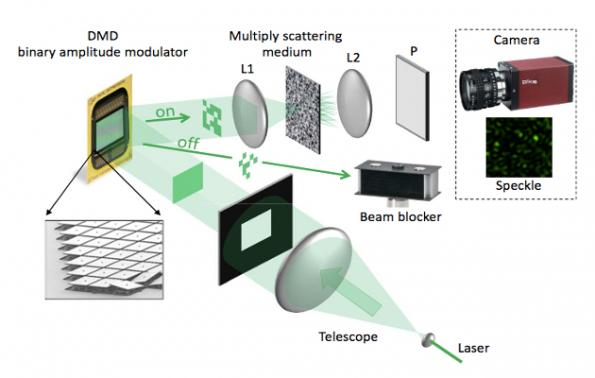
\includegraphics[scale=0.5]{figs/lighton630.jpg}
\end{center}
\caption[OPU's Experimental setup]{OPU's Experimental setup \citep{saade_opu}: A monochromatic laser is expanded by a telescope, then
illuminates a digital micromirror device (DMD), able to spatially encode digital information on the light beam by
amplitude modulation. The light beam carrying the signal is then focused on a random
medium by means of a lens. The transmitted light is collected on the
far side by a second lens, passes through a polarizer, and is measured by a standard monochrome CCD camera for example .}
\label{fig_opu}
\end{figure}
When the incident light is coherent, it promotes complex interference patterns, called speckles, due to the scattering process.
These speckles do not only characterize the propagation medium but also the incident light, and this can be modeled by $y=Wx$, 
where $y$ and $x$ are the vector amplitudes between a set of spatial modes at the output and at the input of the medium respectively. In OPUs, the transmission matrix $W$ of the propagation medium can be approximately considered to be a Gaussian i.i.d matrix. Although it is not explicitely known, it is guaranteed to be stable as long as the propagation medium is stable \citep{saade_opu}.  So using a spatial light modulator and a laser to send an appropriate set of illuminations to the propagation medium, we can acquire the output intensity $|y|^2$ with a CCD or CMOS camera, and that is the principle concept behind OPU's functionality as seen in Fig~ \ref{fig_opu}. To encode a given signal within the incident light, a OPU uses a DMD (digital micromirror device). It is a binary amplitude modulator consisting of an array of micro-mirrors. Each mirror can be activated or not, and thus represent a binary value. %In order to represent grey values, each value is encoded on a square sub-array ($4\times 4$ for example) in the DMD, where the number of lit mirrors reflects the desired level of grey. 
So, generally, a given signal $x$ must be encoded under the form of a binary vector before being passed to the OPU, however we remark that in our case, adjacency matrices of graphlets are already binary, which results in even more speed-up. %The DMD reflects the data and send the reflected light through the disordered medium, then a snapshot of the resulting random projection is acquired using a standard camera.

\subsection{Fast $GSA-\varphi_{OPU}$ algorithm}
One can efficiently deploy the random feature map $\varphi_{OPU}$ in the GSA-$\varphi$ framework, yielding the GSA-$\varphi_{OPU}$ algorithm : it is Algorithm~\ref{alg:GSA} where one uses the random projection $\varphi_{OPU}$ of Eq.~\eqref{OPU_equation} on the vectorized adjacency matrices of each sampled graphlet $F$.
%\begin{algorithm}[H]
%\DontPrintSemicolon
%  \KwInput{2-Classes labelled graph dataset $\mathcal{X}=(\G_i,y_i)_{i=1,\ldots,n}$}
%  \KwOutput{Trained model to classify graphs}
%  \tools{Graph random sampler $S_k$, optical processing unit (OPU), linear classifier (ex. SVM) }\\
%  \Hyp{k:graphlet size, $s$:\#graphlet samples per graph}\\
%  \Algo{\\}
%  Random initialization of the classifier weights\\
%  \For{$\G_i$ in $\mathcal{X}$}{
%  $\boldsymbol{\varphi}_{OPU}(i)=0$\\
%  \For{$j=1:s$}{
%  $F_{i,j}\gets S_k(\G_i)$\\
%  $\mathbf{A}\gets adjacency\_matrix(F_{i,j})$\\
%  $\boldsymbol{\varphi}_{OPU}(i)\gets \boldsymbol{\varphi}_{OPU}(i) +\frac{1}{s}\boldsymbol{\varphi}_{OPU}(F_{i,j})$
%  }
%  }
%  $\mathcal{D}_{\varphi_{OPU}}\gets (\boldsymbol{\varphi}_{OPU}(i),y_i)_{i=1,\ldots, n}$\\
%  Train the linear classifier on the new vector-valued dataset $\mathcal{D}_{\varphi_{OPU}}$
%\caption{GSA-$\varphi_{OPU}$}
%\end{algorithm}
%\todoNK{remove this algorithm}

As mentioned above, the computational cost of $\varphi_{OPU}$ is $\mathcal{O}(1)$, thus independent of both the number of random features and the graphlet size. One can reasonably argue that an OPU has its limits, as the DMD mirror array, where the input $\mathbf{A}$ is encrypted, has a limited dimensions \emph(width $\times$ length). Moreover, the camera used to acquire the light intensity in an OPU has a limited number of pixels thus it introduces a limit on the maximum number of random features. However, within these limits, which are usually large ones, the computational cost is a constant in both $m$ and $k$. 

%To better illustrate the advantage of $GSA-\varphi_{OPU}$ over other discussed methods in this work, we show a table comparing the various theoretical computational times in Table~\ref{table:comp_time}. 

%between them with respect to the computational time per graph $\G$:
%\begin{itemize}
%    \item Graphlet kernel: $C_{gk}= O(\tbinom{v}{k} N_k C_k)$
%    \item Graphlet kernel with sampling: $ C_{gk + gs}= O(C_S s N_k C_k)$
%    \item Gaussian features $GSA_{\varphi_{Gs}}$: $C_{Gs}=O(C_S smk^2)$
%    \item Gaussian features  $GSA_{\varphi_{Gs}}$ with Eigenvalue preprocessing: $C_{Gs+Eig}=O(C_S s(mk+k^3))$
%    \item $GSA_{\varphi_{OPU}}$:  $C_{OPU}=O(C_S s)$
%\end{itemize}

The complexities of the different mappings $\varphi$ examined in this work are summarized in Table \ref{tab:cost}.

\begin{table}
\centering
\begin{tabular}{|c|c|c|c|}
\hline
\multicolumn{2}{|c|}{Graphlet kernel} & \multicolumn{2}{|c|}{$O(\tbinom{v}{k} N_k C^{\cong}_k)$} \\ \hline \hline
%
\multirow{4}{*}{GSA-$\varphi$ with:} & Matching func. $\varphi^{match}_k$ & \multirow{4}{*}{$O(C_S s C_\varphi)$ with $C_\varphi=$ } & $O(N_k C^{\cong}_k)$ \\
& Gaussian RF & & $O(m k^2)$ \\ 
& Gaussian RF on Eig. & & $O(m k + k^3)$ \\ 
& OPU  & & $O(1)$ \\ \hline
\end{tabular}
\caption{Complexities of the different mappings used in GSA-$\varphi$, for a global cost in $O(C_S s C_ \varphi)$.}
\label{tab:cost}
\end{table}

\section{GSA-$\varphi$ concentration inequality proof}
\label{section:proof}

\begin{proof}
Here, we prove theorem \ref{theorem:concentration}. We decompose the proof in two steps.

\paragraph{Step 1: infinite $s$, finite $m$ (number of random features).} Based on our assumption $|\xi_w|\leq 1$, it is a straightforward result of Hoeffding's inequality that  $MMD(\G, \G')^2$ is close to $\frac{1}{m} \sum_{j=1} | \mathbb{E}_{F \sim S_k(\G)} \xi_{\mathbf{w}_j}(F) - \mathbb{E}_{F' \sim S_k(\G')} \xi_{\mathbf{w}_j}(F') |^2 = | \mathbb{E}_{F \sim S_k(\G)} \varphi(F) - \mathbb{E}_{F' \sim S_k(\G')} \varphi(F') |^2$. We recall Hoeffding's inequality below.
\begin{lemma}[Hoeffding's inequality] 
Let $(x_1,\ldots, x_m)$ be independent random variables such that the variable $x_i$ is strictly bounded by the interval $[a_i , b_i]$, and let $\overline{X}=\frac{1}{m}\Sigma_{i=1}^{m}x_i$ then we have:
\begin{equation}
\label{eq:Hoeffding}
    \mathbb{P}(|\mathbb{E}\overline{X}-\overline{X}|\geq \epsilon)\leq 2~ \exp \left(-\frac{2m^2\epsilon^2}{\Sigma_{i=1}^m(b_i-a_i)^2)} \right)
\end{equation}
\end{lemma}
%\begin
In our case, we define the variables $x_j=| \mathbb{E}_{F \sim S_k(\G)} \xi_{\mathbf{w}_j}(F) - \mathbb{E}_{F' \sim S_k(\G')} \xi_{\mathbf{w}_j}(F') |^2$. They are independent, have expectation $MMD(\G,\G')^2$, and are bounded by the interval $[0,4]$, thus we have:
\begin{equation*}
    \mathbb{P}\left(\Big|\frac{1}{m} \sum_{j=1}^m | \mathbb{E}_{F \sim S_k(\G)} \xi_{\mathbf{w}_j}(F) - \mathbb{E}_{F' \sim S_k(\G')} \xi_{\mathbf{w}_j}(F') |^2 - MMD(\G,\G')^2 \Big| \geq \epsilon\right) \leq 2~ e^{ -2m\epsilon^2/16}
\end{equation*}
Or, in other words, with probability $1-\delta$,
\begin{equation}\label{eq:step1}
\Big|\frac{1}{m} \sum_{j=1}^m | \mathbb{E}_{F \sim S_k(\G)} \xi_{\mathbf{w}_j}(F) - \mathbb{E}_{F' \sim S_k(\G')} \xi_{\mathbf{w}_j}(F') |^2 - MMD(\G,\G')^2 \Big| \leq \frac{4 \sqrt{\log (2/\delta)}}{\sqrt{m}}
\end{equation}

\paragraph{Step 2: finite ${s}$ and $m$.} We show that for any \emph{fixed} set of random features $\{\mathbf{w}_j\}$, we have $\| \mathbb{E}_{F \sim S_k(\G)} \varphi(F) - \mathbb{E}_{F' \sim S_k(\G')} \varphi(F')\|$ close to $\| \frac{1}{{s}} \sum_i \varphi(F_i) - \frac{1}{{s}} \sum_i \varphi(F'_i)\|$. 
%Let us consider a fixed set of random variables $\{\omega_j\}_{j \in \{1,\ldots, m\}}$ drawn independently from $\Lambda$, thus the random features map of a graph F equals: $z(F) = \frac{1}{\sqrt{m}}\left[z_{\omega_j}(F)\right]_{j=1}^m$.\newline
By definition of $F_1,\ldots, F_{s}$ random subgraphs drawn independently from $S_k(\G)$, we clearly have: 
\begin{equation}
\label{eq:subsample}
    \mathbb{E}_{F \sim S_k(\G)}~ \varphi(F)= \mathbb{E}\left(~\frac{1}{{s}} \sum_i \varphi(F_i)~\right)
\end{equation} 
Moreover by our assumptions $\varphi(F)$ is in a ball of radius $M=\frac{\sqrt{m}}{\sqrt{m}}=1$. We then apply the following vector version of Hoeffding's inequality.
\begin{lemma}
\label{lemma:vector_hoeffding}
let $X=\{x_1,\ldots,x_{s}\}$ be $iid$ random variables in a ball of radius $M$ centered around the origin in a Hilbert space $\mathcal{H}$. Denote their average by $\overline{X}=\frac{1}{{s}}\sum_{i=1}^{s}x_i$. Then for any $\delta>0$, with probability at lest $1-\delta$, 
\begin{equation}
\label{eq:vector_hoeffding0}
  \| \overline{X}-\mathbb{E}\overline{X}\|_\mathcal{H} \leq \frac{M}{\sqrt{{s}}}\left(1+\sqrt{2\log\frac{1}{\delta}}\right)
\end{equation}
\end{lemma}
\begin{proof}
Although this lemma is well-known in the literature, we reproduce its proof for completeness. Defining the function $f(x)= \| \overline{X}-\mathbb{E}\overline{X}\|$, and $\widetilde{X}={x_1,\ldots,\widetilde{x}_i,\ldots,x_{s}}$ to be a copy of $X$ with the ith element replaced by an arbitrary element of $\mathcal{H}$, we can prove using the triangle inequality:
\begin{equation}
    |f(X)-f(\widetilde{X})|=\Big|\| \overline{X}-\mathbb{E}\overline{X} \|-\|\overline{\widetilde{X}} - \mathbb{E}\overline{X}  \| \Big|\leq \| \overline{X} - \overline{\widetilde{X}}\|\leq
    \frac{\|x_i - \widetilde{x_i} \|}{{s}}\leq
    \frac{2M}{{s}}
\end{equation}
Therefore, $f(X)$ is insensitive to the ith component of $X,~ \forall i \in \{1,\ldots,{s}\}$ which suggests applying McDiarmid's inequality on $f$.

To bound the expectation of $f$, we use the familiar identity about the variance of the average of $iid$ random variables:
\begin{equation}
\mathbb{E}\|\overline{X}-\mathbb{E}\overline{X}\|^2=\frac{1}{n}(\mathbb{E}\|x\|^2-\|\mathbb{E}x\|^2 ) 
\end{equation}
Also:
\[ \mathbb{E}f(X)\leq\sqrt{\mathbb{E}f^2(X)}=\sqrt{\mathbb{E}\|\overline{X}-\mathbb{E}\overline{X}\|^2}\leq \frac{M}{\sqrt{{s}}}\]
This bound for the expectation of $f$ and McDiarmid's inequality give: 
\begin{equation}
\label{eq:vector_hoeffding1}
    \mathbb{P}_x \Big [ f(X)-\frac{M}{\sqrt{{s}}}\geq \epsilon \Big ]\leq
    \mathbb{P}_x \Big [ f(X)-\mathbb{E}f(X)\geq \epsilon \Big ]\leq
    \exp\Big( -\frac{{s}\epsilon^2}{2M^2}\Big)
\end{equation}
Which is equivalent to \eqref{eq:vector_hoeffding0} by setting $\delta=exp( -\frac{{s}\epsilon^2}{2M^2})$ and solving for $\epsilon$.
\end{proof}
Now back to Eq. \eqref{eq:subsample} and its corresponding assumptions that we made, we can directly apply lemma \ref{lemma:vector_hoeffding} (and more specifically Eq.~\eqref{eq:vector_hoeffding1}) to get that with probability $1-\delta$:
\begin{equation}
    \label{eq:fixed_w}
    \left\|\mathbb{E}_{F \sim S_k(\G)} \varphi(F)-~\frac{1}{s} \sum_i \varphi(F_i)~\right\|\geq \frac{1}{\sqrt{{s}}}\left(1+\sqrt{2\log\frac{1}{\delta}}\right)
\end{equation}
Now, by a union bound and triangle inequality: with probability $1-2\delta$,
\begin{align*}
    \Big | \| \mathbb{E}_{F \sim S_k(\G)} \varphi(F)& - \mathbb{E}_{F' \sim S_k(\G')} \varphi(F')\| - \| \frac{1}{{s}} \sum_i \varphi(F_i) - \frac{1}{{s}} \sum_i \varphi(F'_i)\|\Big | \\
    &\leq  \| \mathbb{E}_{F \sim S_k(\G)} \varphi(F) -  \frac{1}{{s}} \sum_i \varphi(F_i) \| + \|\mathbb{E}_{F' \sim S_k(\G')} \varphi(F') - \frac{1}{{s}} \sum_i \varphi(F'_i)\| \\
    &\leq \frac{2}{\sqrt{{s}}}\left(1+\sqrt{2\log\frac{1}{\delta}}\right)
\end{align*}
Moreover, since $\| \mathbb{E}_{F \sim S_k(\G)} \varphi(F)- \mathbb{E}_{F' \sim S_k(\G')} \varphi(F')\| + \| \frac{1}{{s}} \sum_i \varphi(F_i) - \frac{1}{{s}} \sum_i \varphi(F'_i)\| \leq 4$, with the same probability:
\begin{equation}\label{eq:step2}
    \Big | \| \mathbb{E}_{F \sim S_k(\G)} \varphi(F) - \mathbb{E}_{F' \sim S_k(\G')} \varphi(F')\|^2 - \| \frac{1}{{s}} \sum_i \varphi(F_i) - \frac{1}{{s}} \sum_i \varphi(F'_i)\|^2\Big | \leq \frac{8}{\sqrt{{s}}}\left(1+\sqrt{2\log\frac{1}{\delta}}\right)
\end{equation}
%Thus, since the two variables $\| \mathbb{E}_{F \sim f_G} z(F) -  \frac{1}{{s}} \sum_i z(F_i) \|$ and $\|\mathbb{E}_{F' \sim f_{G'}} z(F') - \frac{1}{{s}} \sum_i z(F'_i)\|$ are independent (as a direct result of our aforementioned assumption of independent random sampling), $\forall \epsilon>0$ we have:
%\begin{align*}
%    Pr( \| \mathbb{E}_{F \sim f_G} z(F) -  \frac{1}{{s}} \sum_i z(F_i) \| \geq \frac{1}{\sqrt{{s}}}+\frac{\epsilon}{2}, \|\mathbb{E}_{F' \sim f_{G'}} z(F') - \frac{1}{{s}} \sum_i z(F'_i)\|\geq\frac{1}{\sqrt{{s}}}+\frac{\epsilon}{2})=\\
%    Pr( \| \mathbb{E}_{F \sim f_G} z(F) -  \frac{1}{{s}} \sum_i z(F_i) \| \geq \frac{1}{\sqrt{{s}}}+\frac{\epsilon}{2})~Pr( \|\mathbb{E}_{F' \sim f_{G'}} z(F') - \frac{1}{{s}} \sum_i z(F'_i)\|\geq\frac{1}{\sqrt{{s}}}+\frac{\epsilon}{2})\leq 
%    e^{-\frac{{s}\epsilon^2}{4}}
%\end{align*}
%finally, we get as a straight result from above:
%\begin{align*}
%    Pr(\Big | \| \mathbb{E}_{F \sim f_G} z(F) - \mathbb{E}_{F' \sim f_{G'}} z(F')\| - \| \frac{1}{{s}} \sum_i z(F_i) - \frac{1}{{s}} \sum_i z(F'_i)\|\Big | \geq
%    \frac{2}{\sqrt{{s}}}+\epsilon)\leq e^{-\frac{n\epsilon^2}{4}}
%\end{align*}
%This is true for any fixed set of random variables  $\{w_j\}_{j \in \{1,\ldots, m\}}$ drawn independently from $p(w)$.
Since it is valid for any fixed set of random features, it is also valid with \emph{joint} probability on random features and samples, by the law of total probability.

Finally, combining \eqref{eq:step1}, \eqref{eq:step2}, a union bound and a triangular inequality, we have: with probability $1-3\delta$,
\begin{equation}
\Big|\|\varphi(\mathfrak{F}_\G) - \varphi(\mathfrak{F}_{\G'})\|^2 - MMD(\G,\G')^2 \Big| \leq \frac{4 \sqrt{\log (2/\delta)}}{\sqrt{m}} + \frac{8}{\sqrt{{s}}}\left(1+\sqrt{2\log\frac{1}{\delta}}\right)
\end{equation}
which concludes the proof by taking $\delta$ as $\delta/3$.

\end{proof}



\addchapheadtotoc
\chapter{Results and Discussion}
In this chapter we introduce the experiments conducted in this work  with a discussion of the results. Most of these experiments were on a synthetic graph dataset created based on what's called the stochastic block model (SBM). This generative model is considered since we can control the difficulty of the graph classification problem it introduces and since it is widely used to model real world datasets \citep{SBM}. \newline
One by one, we analyze how our algorithm $GSA-\varphi_{OPU}$, followed by a linear support vector machine model (SVM), is affected by the following parameters: the sampling technique, the number of samples $s$, the graphlet size $k$ and the number of random features $m$.
Then we benchmark this algorithm against state-of-the-art methods: graphlet kernel and graph convolutional networks (GCN). In addition, we benchmark it to $GSA-\varphi_{Gs}$.
In the end, we show some experiments that were done on one real world dataset named \emph{DD} dataset. However, we start now by a general introduction to the generative SBM model. 
\section{Stochastic block model (SBM) dataset}
SBM is commonly known in social sciences to model group structures in friendship graph networks\citep{SBM}. The basic idea here is that nodes  are clustered into many groups, called communities, within the same graph. Then, the neighborhood relations of a node, edges to neighbor nodes, are generated such that nodes in the same community have similar neighbor patterns either to nodes in the same community or to nodes in other communities. \newline
Formally, to generate a graph $\G=(\V,\E)$ of size $v$, the following parameters should be given: The number of communities $\eta$ in the graph, node labels $\{b_1 , \ldots ,b_v\}$ such that node $u$ belongs to community $b_u$, and edge probability matrix $\mathbf{P}=(p_{i,j})_{i,j\in\{1,\ldots, \eta\}}$.
Then the graph is generated by independently adding an edge between any two pair of nodes $(u_1,u_2)$ with probability $p_{b_{u_1} , b_{u_2}}$. \newline
\begin{figure}[H]
\centering
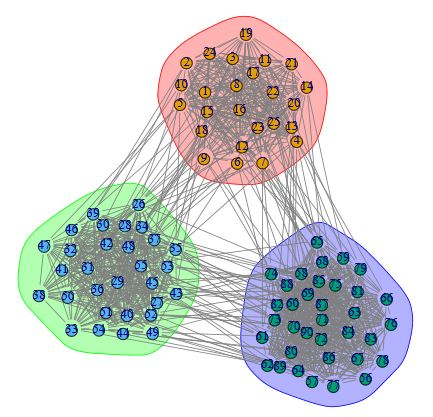
\includegraphics[scale=0.5]{SBM.JPG}
\caption[Visualization of an SBM-based graph example]{An example of a graph generated using SBM model, the graph has 90 nodes divided into three communities of size 25, 30 and 35 nodes. An edge between two nodes within the same community has a probability 0.8, while it has a probability 0.5 if the two nodes belong to different communities.}
%Source:
\label{fig:SBM_example}
\end{figure}
An easy thing to compute here is the average number of edges $\mu$ incident to a node $u$:
\begin{equation}
    \mu_u=\Big[\sum_{b_i\neq b_u} p_{b_u,b_i}*(\#u'\in \V, b_{u'}=b_i \} )\Big]+p_{b_u,b_u}*(\#\{u'\in \V_\G, b_{u'}=b_u \}-1 )
\end{equation}
\subsection{Dataset setup}
In our case and almost in every experiment, unless otherwise mentioned, the SBM dataset consists of 300 graphs, 240 as a training set and 60 as a test set. Each graph has $v=60$ nodes divided equally between six communities $\eta=6$. Moreover, since we are interested in graph 2-classes classification, graphs are divided into two classes based on two different values of the matrix $\mathbf{P}$. But the two matrices have something in common:  $p_{1,1}= p_{2,2} = p_{in}$ and it is obvious that  $p_{1,2}=p_{2,1}=p_{out}$ too, as we want an indirect graphs dataset as indicated previously.\newline
Thus, the first class of graphs corresponds to a fixed pair ($p_{in,1}, p_{out,1}$) and similarly the second   corresponds to ($p_{in,2}, p_{out,2}$). \newline 
In order to prevent the two classes from being easily discriminated by the average degree of nodes in the graph as a feature, the two pairs of probabilities are always chosen so that any node in any graph in any class has the same expected average degree equal to 10. For simplicity, we refer to $r=(p_{in,1}/p_{in,2})$ with inter-classes similarity parameter. Where the closer to one $r$ is, the more similar both classes are, based on the average degree condition,  and thus the harder it is to discriminate them. One notes here that the only parameter that is left to be modified in the experiments is $r$ .


\section{$GSA-\varphi_{OPU}$ behavior with respect to number of samples $s$}
We did two experiments here: the first one is to compare the graphlet distributions introduced by both uniform and random walk sampling, while the second one is to determine the minimum number of samples needed to classify both classes with high test accuracy, or what should be called here validation accuracy.\newline
\subsection{Uniform sampling Vs. random walk sampling}
We generated a graph $\G$ by SBM with a randomly chosen pair $(p_{in},p_{out})$, then we did the following: exhaustive enumeration of all size-5 graphlets in $\G$,  sampling 2000 graphlets of the same size with uniform sampling, then sampling other 2000 graphlets using random walks. For each case, we matched samples to their corresponding graphlet, considering \emph{graphlets without repetition}, to have three graphlet histograms at the end as shown in Fig. \ref{fig:graphlet_hist}. 


\begin{figure}[H]
\centering
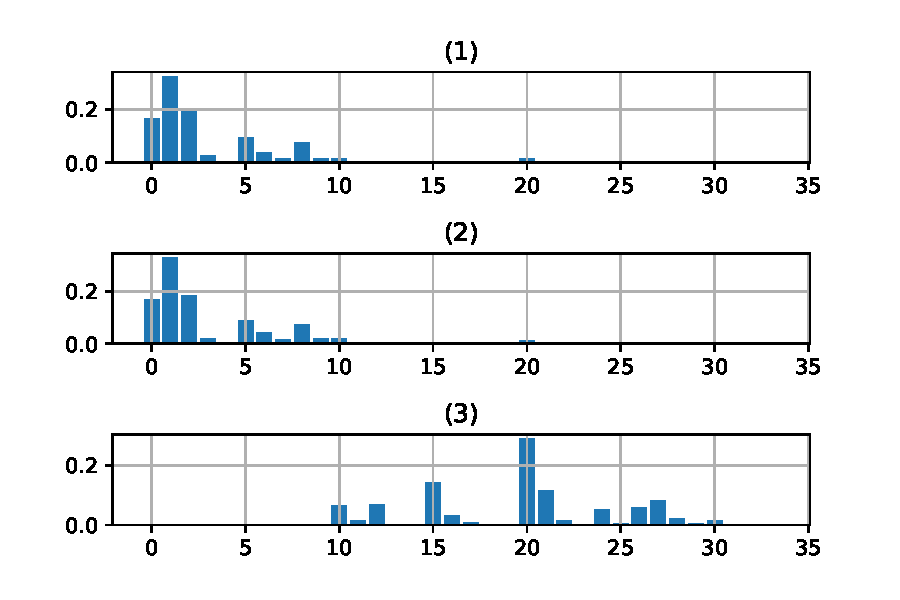
\includegraphics[scale=0.5]{class0_hist.pdf}
\caption[Graphlet histograms of uniform and random walk sampling techniques]{Size-5 graphlet histograms of an SBM random graph, with respecting the isomorphism test. (1): With exhaustive enumeration of all graphlets. (2): 2000 samples with uniform samples. (3): 2000 samples using random walks. }
%Source:
\label{fig:graphlet_hist}
\end{figure}
We see from the results that unlike random walks, uniform sampling is the method to be considered as a sampling technique to approximate graphlet kernel, since it introduces the same histogram as the one used in graphlet kernel. 
\subsection{Varying the number of samples $s$}
experiment setup: number of random features $m=5000$, inter-class similarity $r=2$, input: adjacency matrix $\mathbf{A}$, and sampler: uniform sampling. These parameters were chosen after many experiments to make sure that the 2-classes can be efficiently classified with sufficiently large $s$ and large $k$. Then for graphlet sizes $k\in\{4,5,6\}$, we tried different number of samples and plotted the test accuracy as shown in Fig. \ref{fig:varying_samples_num}.\newline
Results show that even with large number of samples, the algorithm will not perform well if the graphlet size is small as in $k=4$ case. To understand this we can consider the critical case when we use $k=1$ between two graphs, which means that we count how many nodes there are in each. Obviously this is a redundant choice since such graphlets don't provide a lot of information on how nodes are structured and connected in the graph. Thus, for each application, we must choose large $k$ so that graphlets include discriminative patterns not useless ones.
\begin{figure}[H]
\centering
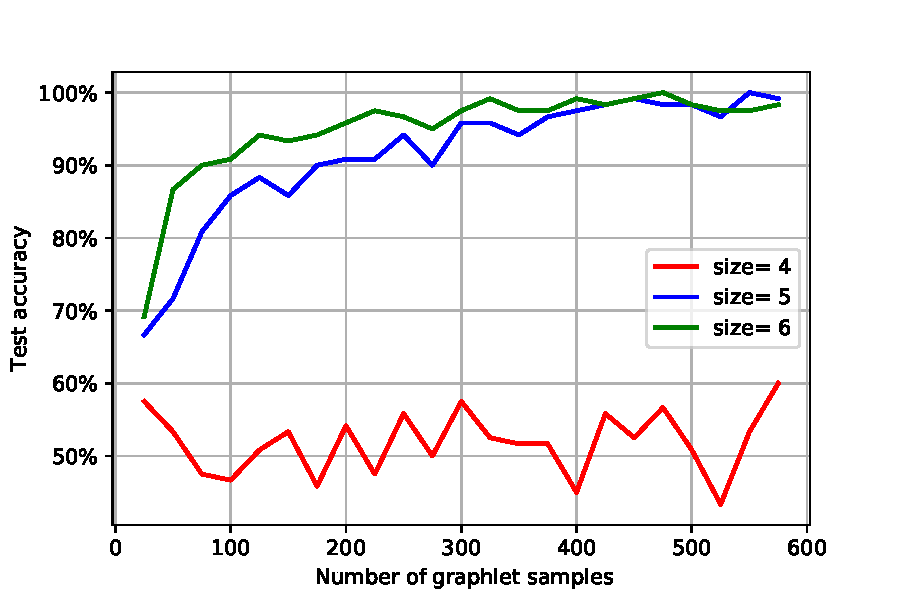
\includegraphics[scale=0.5]{samples_num.pdf}
\caption[$GSA-\varphi_{OPU}$ behavior with respect to number of samples $s$]{$GSA-\varphi_{OPU}$ behavior with respect to number of samples $s$. With $r=2,$, $m=5000$, $k\in\{4,5,6\}$, input: $\mathbf{A}$ and sampler: uniform sampling technique.}
%Source:
\label{fig:varying_samples_num}
\end{figure}
The second note is that in this experiment and even in the next ones, we don't have access to apply the kernel which corresponds to OPUS' random features. That's why we cannot get sure that these results meets the concentration inequalities in chapter\ref{chapter:fast_algorithm}. However, we see that for $k\in\{5,6\}$, test accuracy increases as  $s$ increases, \emph{i.e.} this implies that with higher number of samples $GSA-\varphi_{OPU}$ performance converges to the corresponding mean kernel with higher probability.




\section{$GSA-\varphi_{OPU}$ behavior with respect to the number of random features $m$}
In this experiment we explore the role of random features number $m$ in our algorithm. 
Experiment setup: inter-class similarity: $r=1.1$, graphlet size: $k=6$, sampler: samples number $s=2000$, input: adjacency matrix $\mathbf{A}$, and uniform sampling.
\begin{figure}[H]
\centering
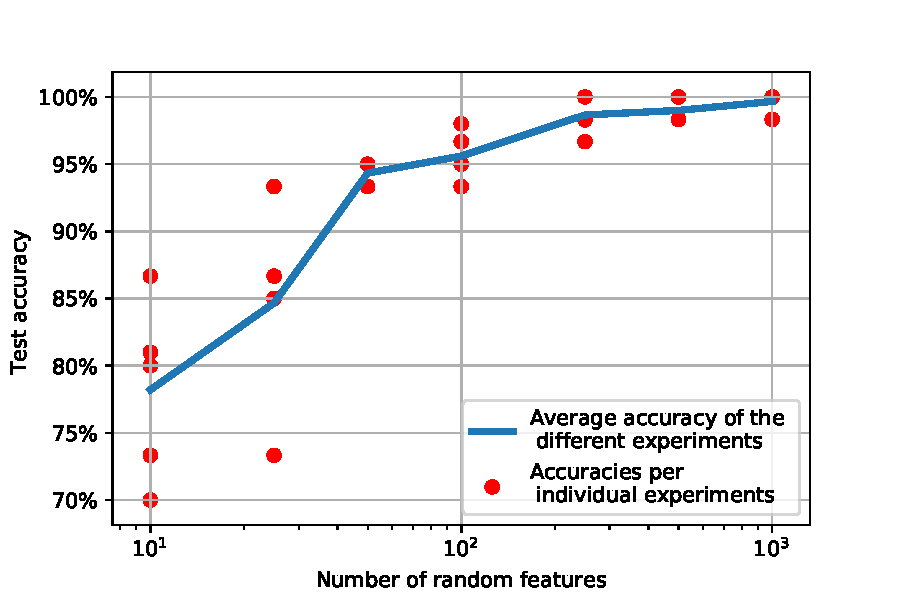
\includegraphics[scale=0.5]{LightON_adj_SBM_varying_RF.PDF}
\caption[$GSA-\varphi_{OPU}$ behavior with respect to number of random features $m$]{$GSA-\varphi_{OPU}$ behavior with respect to number of random features $s$. With  $r=1.1$, $k=6$, $m=5000$, input:$\mathbf{A}$ and sampler: uniform sampling technique. For every value of $m$, the experiment is done five times (red dots), then the $5$ resulted accuracies are averaged (blue curve).}
\label{fig:varying_random_features}
\end{figure}
In addition, for every value of $m$, we applied our algorithm $5$ times on the dataset we have, and then the average of test accuracies is computed. Results are shown in Fig. \ref{fig:varying_random_features}, where we can  see that when $m$ grows, the average test accuracy gets higher, \emph{i.e.} we approximate the performance of the original mean kernel. Even further, as $m$ increases, the 5 experiments provide lower-variance accuracies, which is compatible with the concentration inequalities in chapter \ref{chapter:fast_algorithm}.

\section{testing $GSA-\varphi_{OPU}$ discrimination power}
\begin{figure}[H]
\centering
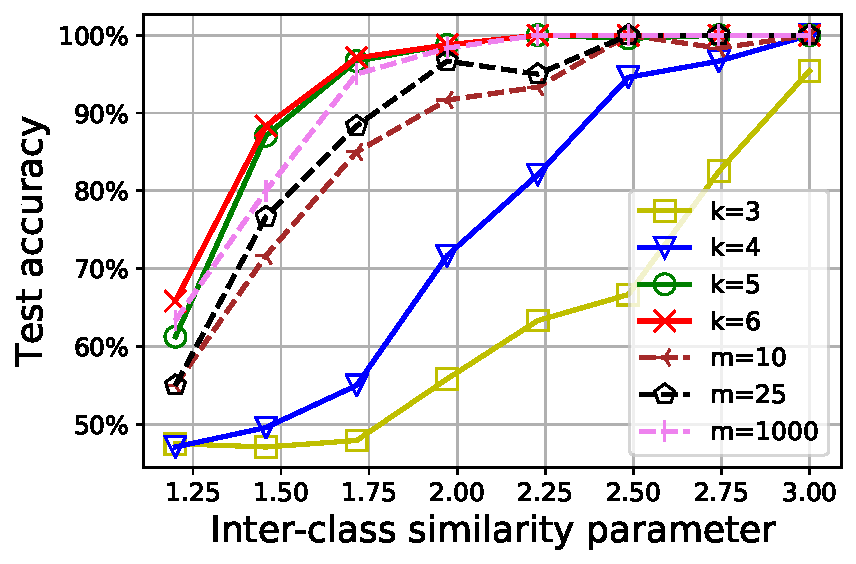
\includegraphics[scale=0.7]{LightOn_adj_SBM_Similarity_graphlet_size.pdf}

\caption[Classification test accuracy as a function of Inter-classes similarity parameter ]{Classification test accuracy with respect to Inter-classes similarity parameter when the number of random features is fixed to 5000 but with different sizes of the graphlet to be sampled. The SVM model is trained on SBM 240-sized labeled dataset. Per graph G, 2000 graphlet samples (Uniform sampling) of the corresponding size are considered to compute its features map $\phi(G)$.}
%Source:
\label{fig:LightOn_adj_SBM_mult_factor}
\end{figure}

\begin{figure}[H]
\centering
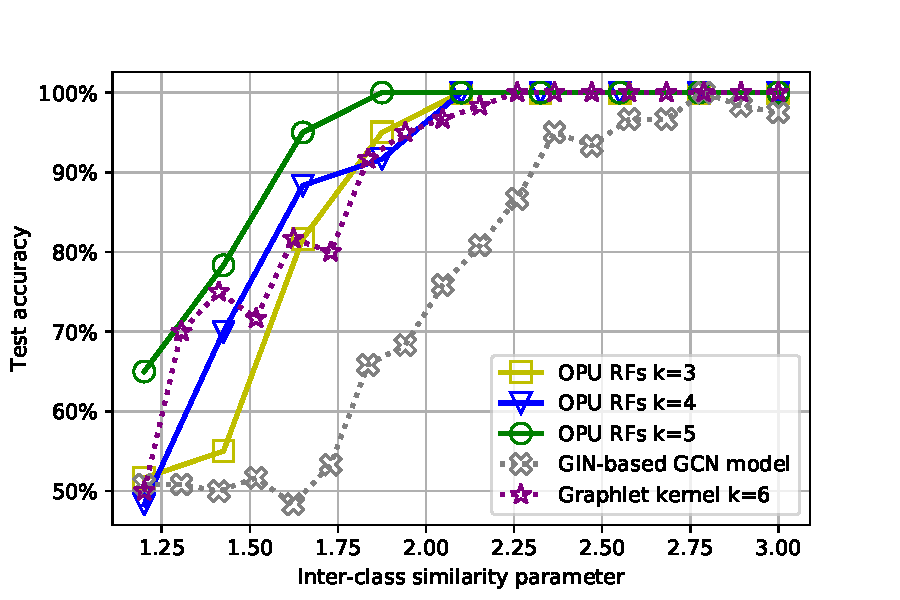
\includegraphics[scale=0.7]{LightOn_adj_SBM_similarity_graphlet_size_RW.pdf}
\caption[Classification test accuracy as a function of Inter-classes similarity parameter ]{Classification test accuracy with respect to Inter-classes similarity parameter when the number of random features is fixed to 5000 but with different sizes of the graphlet to be sampled. The SVM model is trained on SBM 240-sized labeled dataset. Per graph G, 2000 graphlet samples (Random Walk sampling) of the corresponding size are considered to compute its features map $\phi(G)$. This experiment is done to check if the uniform sampling technique is the reason behind the gap between accuracy curves of graphlet sizes 4 and 5 in Fig. \ref{fig:LightOn_adj_SBM_mult_factor} }
%Source:
\label{fig:LightOn_adj_SBM_multfactor_RW}
\end{figure}

\section{Benchmark $GSA-\varphi_{OPU}$ against $GSA-\varphi_{Gs}$}

\section{Benchmark $GSA-\varphi_{OPU}$ against graphlet kernel}
\begin{figure}[H]
\centering
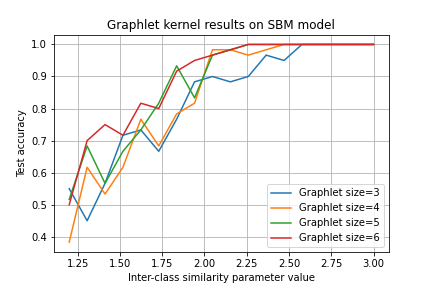
\includegraphics[scale=0.7]{graphlet_kernel_SBM_accuracy.png}
\caption[Graphlet kernel classification test accuracy as a function of Inter-classes similarity parameter]{Graphlet kernel classification test accuracy with respect to Inter-classes similarity parameter $r$. where per graph G, 2000 graphlet samples are considered to compute its graphlet spectrum vector. }
%Source:
\label{fig:graphlet_kernel_SBM}
\end{figure}

\section{Benchmark $GSA-\varphi_{OPU}$ against graph convolution networks}
\begin{figure}[H]
\centering
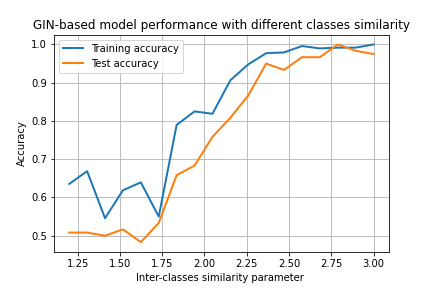
\includegraphics[scale=0.7]{GNN_GIN.png}
\caption[GCN model's classification test accuracy as a function of Inter-classes similarity parameter ]{GCN model's classification test accuracy with respect to Inter-classes similarity parameter. The  model is trained on SBM 240-sized labeled dataset.}
%Source:
\label{fig:GCN_GIN_SBM_multfactor_RW}
\end{figure}

\section{$GSA-\varphi_{OPU}$ results on DD dataset}
\section{Conclusion and future work}







% Bibliography
\begingroup
    \setlength\bibitemsep{10pt}
    \linespread{1}\selectfont
    \printbibliography[title=REFERENCES]
\endgroup
\addcontentsline{toc}{part}{REFERENCES}

% Appendices
%\begin{appendices}
\section{Proof of Theorem 1}\label{app:proof}
\begin{proof} We decompose the proof in two steps.

\textbf{Step 1: infinite $s$, finite $m$.} First we define the random variables $x_j=| \mathbb{E}_{F \sim S_k(\G)} \xi_{\mathbf{w}_j}(F) - \mathbb{E}_{F' \sim S_k(\G')} \xi_{\mathbf{w}_j}(F') |^2$, which are: i/independent, ii/have expectation $MMD(\G,\G')^2$, /iii are bounded by the interval $[0,4]$ based on our assumption $|\xi_w|\leq 1$. Thus, as a straight result of applying  Hoeffding's inequality with easy manipulation: with probability $1-\delta$
\begin{equation}
\label{eq:step1}
\Big|\frac{1}{m} \sum_{j=1}^m x_j- MMD(\G,\G')^2 \Big| \leq\\ \frac{4 \sqrt{\log (2/\delta)}}{\sqrt{m}}
\end{equation}

\textbf{Step 2: finite $s$ and $m$.} For any \emph{fixed} set of random features $\{w_j\}_{1,\ldots,m}$ and based on our previous assumptions we have: i/ $\varphi_{RF}$ is in a ball of radius $M=\frac{\sqrt{m}}{\sqrt{m}}=1$, ii/ $ \mathbb{E}_{F \sim S_k(\G)}~ \varphi(F)= \mathbb{E}\left(~\frac{1}{{s}} \sum_i \varphi(F_i)~\right)$. Therefore, we can directly apply the vector version of Hoeffding's inequality on the vectors $\frac{1}{{s}} \sum_i \varphi(F_i)$ to get that with probability $1-\delta$:
\begin{equation}
    \label{eq:fixed_w}
    \left\|\mathbb{E}_{F \sim S_k(\G)} \varphi(F)-~\frac{1}{s} \sum_i \varphi(F_i)~\right\|\leq \frac{1+\sqrt{2\log\frac{1}{\delta}}}{\sqrt{{s}}}
\end{equation}
\vfill\pagebreak
Defining $J_{exp}(\G,\G')=\| \mathbb{E}_{F \sim S_k(\G)} \varphi(F) - \mathbb{E}_{F' \sim S_k(\G')} \varphi(F')\|$ and $J_{avg}(\G,\G')=\| \frac{1}{{s}} \sum_i \varphi(F_i) - \frac{1}{{s}} \sum_i \varphi(F'_i)\|$, then using triangular inequality followed by a union bound based on \eqref{eq:fixed_w}, we have the following with probability $1-2\delta$,
\begin{align*}
    \Big | J_{exp}(\G,\G') - J_{avg}(\G,\G')\Big | \leq \frac{2}{\sqrt{{s}}}\left(1+\sqrt{2\log\frac{1}{\delta}}\right)
\end{align*}

On the other hand, $ J_{exp}(\G,\G') + J_{avg}(\G,\G')\leq 4$, so with same probability:
\begin{equation}\label{eq:step2}
    \Big | J_{exp}(\G,\G')^2 - J_{avg}(\G,\G')^2 \Big | \leq \frac{8}{\sqrt{{s}}}\left(1+\sqrt{2\log\frac{1}{\delta}}\right)
\end{equation}
Since it is valid for any fixed set of random features, it is also valid with \emph{joint} probability on random features and samples, by the law of total probability.

Finally, combining \eqref{eq:step1}, \eqref{eq:step2} with a union bound and a triangular inequality, we have with probability $1-3\delta$,
\begin{align*}
\Big|\|\varphi(\mathfrak{F}_\G) - \varphi(\mathfrak{F}_{\G'})\|^2 - MMD(\G,\G')^2 \Big| \leq \\\frac{4 \sqrt{\log (2/\delta)}}{\sqrt{m}} + \frac{8}{\sqrt{{s}}}\left(1+\sqrt{2\log\frac{1}{\delta}}\right)
\end{align*}

which concludes the proof by taking $\delta$ as $\delta/3$.

\end{proof}
\end{appendices}

\end{document}
